


\documentclass[a4paper,8pt]{extarticle} % extarticle allows to use font size of 8pt.

\usepackage[a4paper, top=1.6cm, bottom=2cm, left=1.6cm, right=1.6cm]{geometry} % Marge reduction.

%% Language specific package
\usepackage[french]{babel}
\frenchbsetup{StandardLists=true} % Necessary to use enumitem with babel/french.

%% Font and typing packages
\usepackage{fontspec}
\setmainfont[
	Ligatures=TeX,
	ItalicFont={Dancing Script},
	BoldItalicFont={Dancing Script}
	]{PT Serif} % default is Latin Modern
\newfontfamily\antiquefont[Ligatures=TeX]{Caslon Antique} % fancy font
\usepackage{microtype}			% Greatly improves general appearance of the text.
\usepackage{SIunits}			% Unit appearance.
\usepackage{xspace}				% Define commands that appear not to eat spaces.
\usepackage{ulem}				% To cross words out. Use \sout{}.

%% Array utilities
\usepackage{array}				% Additionnal options for arrays.
\usepackage{colortbl}			% Additionnal options for coloring arrays.
\usepackage[table]{xcolor}		% Auto alternate grey-white rows.
\usepackage[export]{adjustbox}		% Centered pics in tables

%% List utilities
\usepackage[inline]{enumitem}   % Display inline lists.
\usepackage{etoolbox}           % General utility. Good for lists for instance.
\usepackage{xparse}             % List utilities.
\usepackage{datatool}	% Handling alphabetical order.

%% Frames
\usepackage{framed}				% Boxes.
\usepackage[framemethod=TikZ]{mdframed}% For fancy frames.
\usepackage{tikz}				% For fancy frames.
\usepackage{wrapfig}			% Fancy insertion of pics in text.

%% Page utilities
\usepackage{multicol}			% Allows to divide a part of the page in multiple columns.
	
%% Others
\usepackage{keyval}             % Used to create maps of commands/labels/objects.
	\makeatletter                  % Mandatory for the usage of keyval.
\usepackage{xstring}            % String parsing, cutting, etc.
\usepackage{hyperref} % Links in PDF.


%%% Update of the dotfill command to always get dots

\newcommand{\predotfill}{\penalty0\hbox{}\nobreak}%


%%% Command to avoid typing \xspace when creating a new name macro

\newcommand{\newnamemacro}[2]{\newcommand{#1}{#2}} % \xspace removed for compatibility with alphabetical ordering

%%% Language specific stuff


\newcommand{\translationteam}{\item \og AEnoriel \fg \item \og Anglachel \fg \item \og Astadriel \fg \item \og Batcat \fg \item \og Bigfish \fg \item \og Eru \fg  \item \og Gandarin \fg \item \og Groumbahk \fg \item \og Iluvatar \fg \item \og Mammstein \fg \item \og Shlagrabak \fg \item et beaucoup d'autres...}

\hypersetup{
	pdfauthor={Équipe de traduction française de T9A},
	pdfsubject={Règles pour le jeu Batailles Fantastiques : Le 9\ieme{} Âge},
}

%%% Commands %%%

\ifdef{\isitanAB}{

\newcommand{\addtosortedlist}[1]{%
	\protected@edef\textarg{#1}%
	\protected@edef\textwithoutspaces{\expandafter\removespaces\expandafter{\textarg}}%
	\substitute\textwithoutspaces{É}{E}% Most used special characters of the language, and equivalent for alphabetical ordering
	\substitute\textwithoutspaces{È}{E}%
	\substitute\textwithoutspaces{Ê}{E}%
	\substitute\textwithoutspaces{é}{e}%
	\substitute\textwithoutspaces{è}{e}%
	\substitute\textwithoutspaces{ê}{e}%
	\substitute\textwithoutspaces{À}{A}%
	\substitute\textwithoutspaces{à}{a}%
	\substitute\textwithoutspaces{ù}{u}%
	\expandafter\sortitem\expandafter[\textwithoutspaces]{#1}%
}%

\newcommand{\pts}[1]{% First step is to remove spaces if there are some
	\def\numberwithoutspaces{\expandafter\removespaces\expandafter{#1}}%
	% Next step is getting rid of formatting if there are any (bold, color, ...)
	\pdfstringdef\cleannumber{\numberwithoutspaces}%
	% Now we can try if it is 1 or not
	\expandafter\ifstrequal\expandafter{\cleannumber}{1}{#1~\labels@point}{%
	\expandafter\ifstrequal\expandafter{\cleannumber}{0.5}{0,5~\labels@point}{%
	\expandafter\ifstrequal\expandafter{\cleannumber}{1.5}{1,5~\labels@point}{%
	#1~\labels@points}}}%
}

}{}

% Dark gods
\newcommand{\dchange}{Changement}
\newcommand{\dlust}{Luxure}
\newcommand{\pestilence}{Pestilence}
\newcommand{\wrath}{Courroux}
\newcommand{\truechaos}{Chaos Primordial}


% Nothing to edit here

\ifdef{\isitanAB}{

\newcommand{\alliancepts}[1]{
\ifsubstring{#1}{\free}{%
		\free{}%
	}{%
	\ifsubstring{#1}{\permodel}{%
		\splitatinf{#1}\myoption\myvalue%
		\pts{\myvalue}\permodel{}%
	}{%
	\pts{#1}
	}}
}

% You might wanna change the order of the gods - advanced user
\newcommand{\allianceoptions}[1]{%
	\defallianceoptions{#1}%
	\unitentryformat{\labels@allianceoptions\spacebeforecolon{}:}\newline
	\expandafter\ifblank\expandafter{\allianceoptions@introsentence}{}{\noindent\allianceoptions@introsentence{}\spacebeforecolon{}:}
	
	\expandafter\ifblank\expandafter{\allianceoptions@wrath}{
		\setlength{\columnseprule}{0.5pt}
		\renewcommand{\columnseprulecolor}{\color{black!30}}
		\vspace*{-0.2cm}\begin{multicols}{3}\raggedcolumns
		
			\begin{center}
			\noindent\dchange{}
			
			\noindent\alliancepts{\allianceoptions@change}
			\vspace*{-0.3cm}
			\end{center}
		
		\columnbreak
		
			\begin{center}
			\noindent\dlust{}
			
			\noindent\alliancepts{\allianceoptions@lust}
			\vspace*{-0.3cm}
			\end{center}
		
		\columnbreak

			\begin{center}
			\noindent\pestilence{}
			
			\noindent\alliancepts{\allianceoptions@pestilence}
			\vspace*{-0.3cm}
			\end{center}
			
		\end{multicols}
		\setlength{\columnseprule}{0pt}	
	}{
		\setlength{\columnseprule}{0.5pt}
		\renewcommand{\columnseprulecolor}{\color{black!30}}
		\vspace*{-0.2cm}\begin{multicols}{4}\raggedcolumns
		
			\begin{center}
			\noindent\dchange{}
			
			\noindent\alliancepts{\allianceoptions@change}
			\vspace*{-0.3cm}
			\end{center}
		
		\columnbreak

			\begin{center}
			\noindent\wrath{}
			
			\noindent\alliancepts{\allianceoptions@wrath}
			\vspace*{-0.3cm}
			\end{center}
		
		\columnbreak
		
			\begin{center}
			\noindent\dlust{}
			
			\noindent\alliancepts{\allianceoptions@lust}
			\vspace*{-0.3cm}
			\end{center}
		
		\columnbreak

			\begin{center}
			\noindent\pestilence{}
			
			\noindent\alliancepts{\allianceoptions@pestilence}
			\vspace*{-0.3cm}
			\end{center}
			
		\end{multicols}
		\setlength{\columnseprule}{0pt}
	}
}

}{}


%%% Labels %%%

% Profile

\newcommand{\labels@M}{M}
\newcommand{\labels@WS}{CC}
\newcommand{\labels@BS}{CT}
\newcommand{\labels@S}{F}
\newcommand{\labels@T}{E}
\newcommand{\labels@W}{PV}
\newcommand{\labels@I}{I}
\newcommand{\labels@A}{A}
\newcommand{\labels@Ld}{Cd}
\newcommand{\labels@Invocation}{Invocation} % For Vampire Covenant profiles
\newcommand{\labels@roundbase}{rond} % printed after XX mm for round bases

\newcommand{\Strength}{Force}

% Technical

\newcommand{\labels@range}{Portée}
\newcommand{\labels@point}{pt}
\newcommand{\labels@points}{pts}
\newcommand{\labels@only}{uniquement}
\newcommand{\labels@magic}{Magie}
\newcommand{\labels@pathsused}{Génère ses sorts dans la Discipline}
\newcommand{\labels@model}{figurine}
\newcommand{\labels@models}{figurines}
\newcommand{\labels@Singlemodel}{Figurine \textbf{seule}}

% Unit entry labels

\newcommand{\labels@basesize}{Socle}
\newcommand{\labels@trooptype}{Type de troupe}
\newcommand{\labels@specialrules}{Règles Spéciales}
\newcommand{\labels@alignment}{Allégeance}
\newcommand{\labels@alliance}{Allégeance}
\newcommand{\labels@allianceoptions}{Options d'Allégeance}
\newcommand{\labels@greenhiderace}{Race de Peaux Vertes}
\newcommand{\labels@equipment}{Équipement}
\newcommand{\labels@weapons}{Armes}
\newcommand{\labels@armour}{Armure}
\newcommand{\labels@options}{Options}
\newcommand{\labels@commandgroup}{État-Major}
\newcommand{\labels@charactermounts}{Montures de Personnages}
\newcommand{\labels@mounts}{Montures}
\newcommand{\labels@mount}{Monture}
\newcommand{\labels@specialequipment}{Équipement Spécial}

% Command groups

\newcommand{\labels@champion}{Champion}
\newcommand{\labels@standardbearer}{Porte-Étendard}
\newcommand{\labels@musician}{Musicien}
\newcommand{\labels@singlebannerallowance}{Une seule unité de ce type peut prendre une Bannière Magique}
\newcommand{\labels@condsinglebannerallowance}{Une seule unité de ce type peut prendre une Bannière Magique si}
\newcommand{\labels@bannerallowance}{Bannière Magique}
\newcommand{\labels@veteranstandardbearer}{Peut devenir Porte-Étendard Vétéran}
\newcommand{\labels@championallowance}{Arme Magique}

% Titles

\newcommand{\labels@armylist}{Liste des Troupes}
\newcommand{\labels@lords}{Seigneurs}
\newcommand{\labels@heroes}{Héros}
\newcommand{\labels@coreunits}{Unités de Base}
\newcommand{\labels@specialunits}{Unités Spéciales}
\newcommand{\labels@rareunits}{Unités Rares}
\newcommand{\labels@armywiderules}{Règles Communes de l'Armée}
\newcommand{\labels@armyspecialrules}{Règles Spéciales de l'Armée}
\newcommand{\labels@armoury}{Armurerie}
\newcommand{\labels@magicalitems}{Objets Magiques}
\newcommand{\labels@magicalweapons}{Armes Magiques}
\newcommand{\labels@magicalarmour}{Armures Magiques}
\newcommand{\labels@talismans}{Talismans}
\newcommand{\labels@enchanteditems}{Objets Enchantés}
\newcommand{\labels@arcaneitems}{Objets Cabalistiques}
\newcommand{\labels@magicalbanners}{Bannières Magiques}
\newcommand{\labels@quickrefsheet}{Fiche de Référence}
\newcommand{\labels@changelog}{Change Log}

\newcommand{\labels@lordsInitial}{S}
\newcommand{\labels@heroesInitial}{H}
\newcommand{\labels@coreunitsInitial}{B}
\newcommand{\labels@specialunitsInitial}{S}
\newcommand{\labels@rareunitsInitial}{R}
\newcommand{\labels@mountsInitial}{M}


% Titlepage

\newcommand{\labels@fantasybattles}{Batailles Fantastiques}
\newcommand{\labels@NinthAge}{Le 9\ieme{} Âge}
\newcommand{\labels@armyrules}{Règles de l'Armée}
\newcommand{\labels@frontpagecredits}{%
\labels@fantasybattles{} : \labels@NinthAge{} est un jeu créé et entretenu par la communauté qui met en scène des affrontements de figurines.\newline
Toutes les règles sont disponibles gratuitement sur le site suivant. Vos retours et suggestions sont les bienvenus : \url{http://www.the-ninth-age.com/}
}
\newcommand{\labels@license}{Copyright Creative Commons license : \url{the-ninth-age.com/license.html}}
\newcommand{\labels@tableofcontents}{Sommaire}
\newcommand{\labels@introduction}{%
\begin{center}\noindent{\Largerfontsize\textbf{Note des traducteurs}}\end{center}
\vspace{0.5cm}

Nous souhaitons remercier chaleureusement l'équipe à l'initiative du 9\ieme{} Âge pour leur motivation et leur travail continu pour faire vivre notre passion. Nous espérons que ce jeu saura développer les qualités pour plaire au plus grand nombre et réunir les joueurs, amateurs comme habitués des tournois, autour de règles amusantes et équilibrées, pour finalement s'imposer comme un standard du jeu de figurines. Une grande ambition qui ne pourra s'accomplir que \textbf{grâce à vous}, la communauté, via des retours constructifs, afin de modeler le jeu selon nos désirs. N'étant \textbf{en aucun cas à but lucratif}, le 9\ieme{} Âge part avec un avantage considérable. Les règles des éventuelles nouvelles sorties ne sont pas dictées par le besoin de vendre ces nouveautés. Vous pouvez choisir et acheter vos figurines où bon vous semble, il n'y a pas un unique revendeur toléré. Enfin, vous pouvez être assurés que tant que le 9\ieme{} Âge sera joué, vous disposerez d'un \textbf{support continu et régulier}, celui-ci étant offert par la communauté.

Concernant la traduction en elle-même, nous avons fait de notre mieux pour vous offrir une version de qualité, dont nous espérons qu'elle surpasse celle de la version originale ! Si vous constatez des coquilles, des erreurs, merci de nous les signaler en nous contactant sur le forum du 9\ieme{} Âge, dans le \textbf{sous-forum français} (\url{http://www.the-ninth-age.com/index.php?board/117-french/}). Vous y trouverez aussi les dernières mises à jour. \textbf{En cas de conflit d'interprétation avec la version originale, la version originale fait référence}.

\vspace{0.5cm}
Que ce jeu vous apporte d'innombrables heures de plaisir partagé !

\vspace{1cm}

\ifdef{\translationteam}{
	\begin{multicols}{3}
	\begin{itemize}
		\translationteam
	\end{itemize}
	\end{multicols}
}{}
}
\newcommand{\labels@rulechanges}{% blank ATM
}
\newcommand{\labels@latexcredit}{Document réalisé à l'aide de \LaTeX .}


%%% Technical commands

\newcommand{\only}[1]{(#1 uniquement)}
\newcommand{\free}{gratuit}
\newcommand{\upto}{jusqu'à}
\newcommand{\Upto}{Jusqu'à}
\newcommand{\unlimited}{pas de limite}
\newcommand{\permodel}{/fig.}
\newcommand{\listlastchoice}{ ou}
\newcommand{\notif}[1]{(pas #1)}
\newcommand{\wordand}{et}
\newcommand{\wordwith}{avec}
\newcommand{\ifNmodelsorless}[1]{(#1 figurines ou moins)}
\newcommand{\unitwith}{unité avec}
\newcommand{\From}{De} % From ... to ... models
\newcommand{\wordto}{à}
\newcommand{\wordAll}{Tous}
\newcommand{\spacebeforecolon}{ } % French put a space before colons
\newcommand{\minprice}{Coût min. :}
\newcommand{\mincostfor}{Coût min. pour}
\newcommand{\maxunitsize}{Taille max.}
\newcommand{\additionalfigscost}{Les figurines additionnelles coûtent}


%%% Special rules %%%

\newcommand{\ambush}{Embuscade}
\newcommand{\armourpiercing}[1]{Perforant\ifblank{#1}{}{ (#1)}}
\newcommand{\bodyguard}[1]{Garde du Corps\ifblank{#1}{}{ (#1)}}
\newcommand{\breathweapon}[1]{Attaque de Souffle\ifblank{#1}{}{ (#1)}}
\newcommand{\channel}{Canalisation}
\newcommand{\crushattack}{Attaque Écrasante}
\newcommand{\daemonicinstability}{Instabilité Démoniaque}
\newcommand{\devastatingcharge}{Charge Dévastatrice}
\newcommand{\distracting}{Distrayant}
\newcommand{\divineattacks}{Attaques Divines}
\newcommand{\engineer}{Ingénieur}
\newcommand{\ethereal}{Éthéré}
\newcommand{\fastcavalry}{Cavalerie Légère}
\newcommand{\fear}{Peur}
\newcommand{\fightinextrarank}{Combat avec un Rang Supplémentaire}
\newcommand{\fireborn}{Né du Feu}
\newcommand{\flamingattacks}{Attaques Enflammées}
\newcommand{\flammable}{Inflammable}
\newcommand{\frenzy}{Frénésie}
\newcommand{\fly}[1]{Vol\ifblank{#1}{}{ (#1)}}
\newcommand{\grindingattacks}[1]{Attaques de Broyage\ifblank{#1}{}{ (#1)}}
\newcommand{\hardtarget}{Camouflé}
\newcommand{\hatred}{Haine}
\newcommand{\hellfire}{Feu Démoniaque}
\newcommand{\hidden}{Caché}
\newcommand{\holyattacks}{Attaques Divines} % deprecated, still has to be filled. same as Divine Attacks.
\newcommand{\immunetopsychology}{Immunisé à la Psychologie}
\newcommand{\impacthits}[1]{Touches d'Impact\ifblank{#1}{}{ (#1)}}
\newcommand{\insignificant}{Insignifiant}
\newcommand{\largetarget}{Grande Cible}
\newcommand{\lethalstrike}{Coup Fatal}
\newcommand{\lightningattacks}{Attaques Foudroyantes}
\newcommand{\lightningreflexes}{Réflexes Foudroyants}
\newcommand{\lighttroops}{Troupe Légère}
\newcommand{\magicresistance}[1]{Résistance à la Magie\ifblank{#1}{}{ (#1)}}
\newcommand{\magicalattacks}{Attaques Magiques}
\newcommand{\metalshifting}{Fusion du Métal}
\newcommand{\moveorfire}{Mouvement ou Tir}
\newcommand{\multipleshots}[1]{Tirs Multiples\ifblank{#1}{}{ (#1)}}
\newcommand{\multiplewounds}[2]{Blessures Multiples\ifblank{#1}{}{ (#1\ifblank{#2}{)}{, #2)}}}
\newcommand{\notaleader}{Pas un Meneur}
\newcommand{\otherworldly}{D'Outre-Monde}
\newcommand{\pathmaster}[1]{Maître de la Voie\ifblank{#1}{}{ (#1)}}
\newcommand{\poisonedattacks}{Attaques Empoisonnées}
\newcommand{\quicktofire}{Tir Rapide}
\newcommand{\randommovement}[1]{Mouvement Aléatoire\ifblank{#1}{}{ (#1)}}
\newcommand{\randomattacks}[1]{Attaques Aléatoires\ifblank{#1}{}{ (#1)}}
\newcommand{\regeneration}[1]{Régénération\ifblank{#1}{}{ (#1+)}}
\newcommand{\reload}{Rechargez !}
\newcommand{\requirestwohands}{Arme à deux Mains}
\newcommand{\scythes}{Faux}
\newcommand{\scout}{Éclaireur}
\newcommand{\scouts}{Éclaireurs}
\newcommand{\stomp}[1]{Piétinement\ifblank{#1}{}{ (#1)}}
\newcommand{\strider}[1]{Guide\ifblank{#1}{}{ (#1)}}
\newcommand{\stubborn}{Tenace}
\newcommand{\stupidity}{Stupidité}
\newcommand{\skirmisher}{Tirailleur}
\newcommand{\skirmishers}{Tirailleurs}
\newcommand{\sweepingattack}{Attaque au Passage}
\newcommand{\swiftstride}{Course Rapide}
\newcommand{\thunderouscharge}{Charge Tonitruante}
\newcommand{\terror}{Terreur}
\newcommand{\toxicattacks}{Attaques Toxiques}
\newcommand{\unbreakable}{Indémoralisable}
\newcommand{\undead}{Mort-Vivant}
\newcommand{\unstable}{Instable}
\newcommand{\unwieldy}{Encombrant}
\newcommand{\vanguard}{Avant-Garde}
\newcommand{\volleyfire}{Tir de Volée}
\newcommand{\warplatform}{Plateforme de Guerre}
\newcommand{\wardsave}[1]{Sauvegarde Invulnérable\ifblank{#1}{}{ (#1+)}}
\newcommand{\weaponmaster}{Maître d'Ar\-mes}
\newcommand{\wizardconclave}[1]{Conclave de Sorciers\ifblank{#1}{}{ (#1)}}


%%% Magic %%%


% General

\newcommand{\Pathof}{Voie}

\newcommand{\battle}{Commune}

\newcommand{\anyofthebattlemagic}{dans n'importe laquelle des Voies Communes}
\newcommand{\ONLYanyofthebattlemagic}{Commune de votre choix}

\newcommand{\magiclevel}[1]{\ifnumcomp{#1}{<}{3}{Apprenti Magicien}{Maître Magicien} Niveau #1}
\newcommand{\Level}{Niveau}

\newcommand{\wizard}{Magicien}
\newcommand{\wizards}{Magiciens}

\newcommand{\learnedspell}{Sort Appris}
\newcommand{\learnedspells}{Sorts Appris}
\newcommand{\attributespell}{Attribut de la Voie}
\newcommand{\attributespells}{Attributs de la Voie}
\newcommand{\attributespellnumber}{A}
\newcommand{\traitspell}{Sort Caractéristique}
\newcommand{\traitspells}{Sorts Caractéristiques}
\newcommand{\traitspellnumber}{C}


\newcommand{\boundspell}[1]{Objet de Sort\ifblank{#1}{}{, Puissance #1}}
\newcommand{\boundspells}[1]{Objets de Sort\ifblank{#1}{}{, Puissance #1}}

% Casting Vocabulary

\newcommand{\lostfocus}{Perte de Concentration}
\newcommand{\miscast}{Fiasco}
\newcommand{\miscasts}{Fiascos}
\newcommand{\overwhelmingpower}{Pouvoir Irrésistible}

\newcommand{\breachintheveil}{Brèche dans le Voile}
\newcommand{\catastrophicdetonation}{Explosion Catastrophique}
\newcommand{\witchfire}{Feu de Sorcières}
\newcommand{\sorcerousbacklash}{Contrecoup Magique}
\newcommand{\amnesia}{Amnésie}

% Spell Types

\newcommand{\augment}{Amélioration}
\newcommand{\hex}{Malédiction}
\newcommand{\universal}{Universel}
\newcommand{\missile}{Projectile}
\newcommand{\damage}{Dégâts}
\newcommand{\direct}{Direct}
\newcommand{\focused}{Focalisé}
\newcommand{\vortex}{Vortex}
\newcommand{\ground}{Marqueur}
\newcommand{\linetemplate}{Gabarit de Ligne}
\newcommand{\specialTYPE}{Spécial}
\newcommand{\aura}{Aura}
\newcommand{\castersunit}{Unité du Lanceur}
\newcommand{\caster}{Lanceur}

\newcommand{\template}{Gabarit}

% Spell Durations

\newcommand{\lastsoneturn}{Dure un Tour}
\newcommand{\instant}{Immédiat}
\newcommand{\permanent}{Permanent}
\newcommand{\remainsinplay}{Reste en Jeu}


% Battle Magic

\newcommand{\alchemy}{de l'Alchimie}
\newcommand{\alchemyattribute}{Édit de Fer}
\newcommand{\alchemysignature}{Métal Fondu}
\newcommand{\alchemyspellone}{Lames Enchantées}
\newcommand{\alchemyspelltwo}{Corrosion Rampante}
\newcommand{\alchemyspellthree}{Manteau de Vif-Argent}
\newcommand{\alchemyspellfour}{Pieu d'Argent}
\newcommand{\alchemyspellfive}{Fléau de l'Acier}
\newcommand{\alchemyspellsix}{Transmutation en Or}

\newcommand{\death}{de la Mort}
\newcommand{\deathattribute}{Nuage de Désespoir}
\newcommand{\deathsignature}{Le Baiser de la Faucheuse}
\newcommand{\deathspellone}{Malédiction du Mortel}
\newcommand{\deathspelltwo}{Esprits Dévorants}
\newcommand{\deathspellthree}{Sangsue Psychique}
\newcommand{\deathspellfour}{Moisson d’Âmes}
\newcommand{\deathspellfive}{L’Abîme aussi te Regarde...}
\newcommand{\deathspellsix}{Maelström d’Âmes}

\newcommand{\fire}{du Feu}
\newcommand{\fireattribute}{Feu Déchaîné}
\newcommand{\firesignature}{Boule de Feu}
\newcommand{\firespellone}{Cascade Ardente}
\newcommand{\firespelltwo}{Épées Flamboyantes}
\newcommand{\firespellthree}{Jet de Flammes}
\newcommand{\firespellfour}{Traits Enflammés}
\newcommand{\firespellfive}{Remparts Incandescents}
\newcommand{\firespellsix}{Souffler sur les Braises}

\newcommand{\heavens}{des Cieux}
\newcommand{\heavensattribute}{Second Sceau}
\newcommand{\heavenssignature}{Aquilon}
\newcommand{\heavensspellone}{Bourrasque}
\newcommand{\heavensspelltwo}{Choc Foudroyant}
\newcommand{\heavensspellthree}{Conjonction Astrale}
\newcommand{\heavensspellfour}{Fléau du Ponant}
\newcommand{\heavensspellfive}{Déluge d'Éclairs}
\newcommand{\heavensspellsix}{Appel de la Comète}

\newcommand{\light}{de la Lumière}
\newcommand{\lightattribute}{Lumière Gardienne}
\newcommand{\lightsignature}{Éclat Brûlant}
\newcommand{\lightspellone}{Bouclier Protecteur}
\newcommand{\lightspelltwo}{Étincelle de Courage}
\newcommand{\lightspellthree}{Vitesse Fulgurante}
\newcommand{\lightspellfour}{Toile Scintillante}
\newcommand{\lightspellfive}{Distorsion Temporelle}
\newcommand{\lightspellsix}{Bannissement Divin}

\newcommand{\nature}{de la Nature}
\newcommand{\natureattribute}{Souffle de Vie}
\newcommand{\naturesignature}{Eaux Vivifiantes}
\newcommand{\naturespellone}{Maître de la Terre}
\newcommand{\naturespelltwo}{Le Trône de Chêne}
\newcommand{\naturespellthree}{Esprits des Bois}
\newcommand{\naturespellfour}{Croissance Estivale}
\newcommand{\naturespellfive}{Peau Rocailleuse}
\newcommand{\naturespellsix}{Créatures Souterraines}

\newcommand{\shadows}{des Ombres}
\newcommand{\shadowsattribute}{Course Parmi les Ombres}
\newcommand{\shadowssignature}{Miasmes Obscurs}
\newcommand{\shadowsspellone}{Orbe de Noirceur}
\newcommand{\shadowsspelltwo}{Partir en Fumée}
\newcommand{\shadowsspellthree}{Expérience de Mort Imminente}
\newcommand{\shadowsspellfour}{Char Vaporeux}
\newcommand{\shadowsspellfive}{Ombres Dévorantes}
\newcommand{\shadowsspellsix}{Scalpel Psychique}

\newcommand{\wilderness}{de la Sauvagerie}
\newcommand{\wildernessattribute}{La Chasse Sauvage}
\newcommand{\wildernesssignature}{La Bête qui Sommeille}
\newcommand{\wildernessspellone}{Essaim d’Insectes}
\newcommand{\wildernessspelltwo}{Rage Intérieure}
\newcommand{\wildernessspellthree}{Pieu de Rougebois}
\newcommand{\wildernessspellfour}{Calamité des Bois Sauvages}
\newcommand{\wildernessspellfive}{Tempête Furieuse}
\newcommand{\wildernessspellsix}{Métamorphose
Monstrueuse}

\newcommand{\eightpaths}{Octuple}



% Army Specific Magic

\newcommand{\butchery}{de la Boucherie}
\newcommand{\butcheryattribute}{Sang de Kholag}
\newcommand{\butcherysignature}{Briseur de Dents}
\newcommand{\butcheryspellone}{Buveur de Moelle}
\newcommand{\butcheryspelltwo}{Festin de Tripaille}
\newcommand{\butcheryspellthree}{Concasseur d’Os}
\newcommand{\butcheryspellfour}{Gobeur de Cervelle}
\newcommand{\butcheryspellfive}{Cœur de Troll}
\newcommand{\butcheryspellsix}{Gosier de Géant}

\newcommand{\change}{du Changement}
\newcommand{\changeattribute}{Vent du Changement}
\newcommand{\changesignature}{Feu Azur}
\newcommand{\changespellone}{Feu Rose}
\newcommand{\changespelltwo}{Vague du Changement}
\newcommand{\changespellthree}{Secrets Volés}
\newcommand{\changespellfour}{Règne de la Confusion}
\newcommand{\changespellfive}{Inéluctable Trahison}
\newcommand{\changespellsix}{Portail Éternel}

\newcommand{\thebiggreengods}{des Grands Dieux Verts}
\newcommand{\thebiggreengodsattribute}{Chopez-les !}
\newcommand{\thebiggreengodssignature}{L'Heure de la Raclée}
\newcommand{\thebiggreengodsspellone}{Coup de Boule}
\newcommand{\thebiggreengodsspelltwo}{Poings Bastonneurs}
\newcommand{\thebiggreengodsspellthree}{Même Pas Mal !}
\newcommand{\thebiggreengodsspellfour}{Grande Main Verte}
\newcommand{\thebiggreengodsspellfive}{Boum !}
\newcommand{\thebiggreengodsspellsix}{Le Gros Piétinement}

\newcommand{\thelittlegreengods}{des Petits Dieux Verts}
\newcommand{\thelittlegreengodsattribute}{Fourbe Larcin}
\newcommand{\thelittlegreengodssignature}{Œil Mauvais}
\newcommand{\thelittlegreengodsspellone}{Taillades Sournoises}
\newcommand{\thelittlegreengodsspelltwo}{Bénédiction de la Mère-Araignée}
\newcommand{\thelittlegreengodsspellthree}{Ça Démange ?}
\newcommand{\thelittlegreengodsspellfour}{Chut ! Pas un Bruit...}
\newcommand{\thelittlegreengodsspellfive}{J’vous Arrange Ça}
\newcommand{\thelittlegreengodsspellsix}{Malédiction de la Lune Verte}

\newcommand{\blackmagic}{de la Magie Noire}
\newcommand{\blackmagicattribute}{Soif d’Âmes}
\newcommand{\blackmagicsignature}{Furie de Moraec}
\newcommand{\blackmagicspellone}{Rafale Glaciale}
\newcommand{\blackmagicspelltwo}{Tourbillon de Lames}
\newcommand{\blackmagicspellthree}{Agonie Paralysante}
\newcommand{\blackmagicspellfour}{Marque de la Peur}
\newcommand{\blackmagicspellfive}{Trait d’Énergie Noire}
\newcommand{\blackmagicspellsix}{Terreur Noire}

\newcommand{\disease}{de la Maladie}
\newcommand{\diseaseattribute}{Bénédiction Nécrotique}
\newcommand{\diseasesignature}{Relents de Pestilence}
\newcommand{\diseasespellone}{Haleine Corruptrice}
\newcommand{\diseasespelltwo}{Toucher Putréfiant}
\newcommand{\diseasespellthree}{Excroissance Adipeuse}
\newcommand{\diseasespellfour}{Purge Parasitaire}
\newcommand{\diseasespellfive}{Malédiction du Lépreux}
\newcommand{\diseasespellsix}{Tourbillon Fétide}

\newcommand{\lust}{de la Luxure}
\newcommand{\lustattribute}{Masochisme}
\newcommand{\lustsignature}{Flagellation Démoniaque}
\newcommand{\lustspellone}{Grâce Hypnotique}
\newcommand{\lustspelltwo}{Valse Irrésistible}
\newcommand{\lustspellthree}{Hystérie}
\newcommand{\lustspellfour}{Fantasmagorie}
\newcommand{\lustspellfive}{Déchirement psychique}
\newcommand{\lustspellsix}{Chœur Dissonant}

\newcommand{\necromancy}{de la Nécromancie}
\newcommand{\necromancyattribute}{Tromper la Faucheuse}
\newcommand{\necromancysignature}{Adjuration des Morts}
\newcommand{\necromancyspellone}{Parodie de Vie}
\newcommand{\necromancyspelltwo}{Convocation Profanatoire}
\newcommand{\necromancyspellthree}{Sarabande Macabre}
\newcommand{\necromancyspellfour}{Regard de Setesh}
\newcommand{\necromancyspellfive}{Vol de Jeunesse}
\newcommand{\necromancyspellsix}{Malédiction des Morts}

\newcommand{\ruin}{de la Ruine}
\newcommand{\ruinattribute}{Hordes Sans Fin}
\newcommand{\ruinsignature}{Éclair Noir}
\newcommand{\ruinspellone}{Nourrissons-les...}
\newcommand{\ruinspelltwo}{Souiller le Sol}
\newcommand{\ruinspellthree}{La Faim}
\newcommand{\ruinspellfour}{Appel de la Tempête}
\newcommand{\ruinspellfive}{Rupture Sismique}
\newcommand{\ruinspellsix}{Pour Qui Sonne le Glas}

\newcommand{\forge}{de la Forge}
\newcommand{\forgeattribute}{Fournaise Haineuse}
\newcommand{\forgesignature}{Bouclier de Sombrefeu}
\newcommand{\forgespellone}{Rage Incendiaire}
\newcommand{\forgespelltwo}{Subjugation}
\newcommand{\forgespellthree}{Souffle de Haine}
\newcommand{\forgespellfour}{Anathème de Noirceur}
\newcommand{\forgespellfive}{Cendres Asphyxiantes}
\newcommand{\forgespellsix}{Flammes de la Forge}

\newcommand{\sands}{des Sables}
\newcommand{\sandsattribute}{Les Morts sans Repos}
\newcommand{\sandssignature}{Sirocco}
\newcommand{\sandsspellone}{Lames Maudites}
\newcommand{\sandsspelltwo}{Dessiccation Mortelle}
\newcommand{\sandsspellthree}{Frappes Vengeresses}
\newcommand{\sandsspellfour}{Jugement Divin}
\newcommand{\sandsspellfive}{Sables Mouvants}
\newcommand{\sandsspellsix}{Écho des Gloires
Passées}

\newcommand{\whitemagic}{de la Magie Blanche}
\newcommand{\whitemagicattribute}{Bouclier des Anciens}
\newcommand{\whitemagicsignature}{Traits de Lumière}
\newcommand{\whitemagicspellone}{Résurrection du Phénix}
\newcommand{\whitemagicspelltwo}{Volonté Inspirante}
\newcommand{\whitemagicspellthree}{Sentier Secret}
\newcommand{\whitemagicspellfour}{Bénédiction d’Amhar}
\newcommand{\whitemagicspellfive}{Fusion d’Artefact}
\newcommand{\whitemagicspellsix}{Cataclysme}

% Paths Initials

\newcommand{\alchemyInitials}{A}
\newcommand{\deathInitials}{M}
\newcommand{\fireInitials}{F}
\newcommand{\heavensInitials}{C}
\newcommand{\lightInitials}{L}
\newcommand{\natureInitials}{N}
\newcommand{\shadowsInitials}{O}
\newcommand{\wildernessInitials}{S}

\newcommand{\eightfoldInitials}{8}

\newcommand{\whitemagicInitials}{MB}
\newcommand{\blackmagicInitials}{MN}
\newcommand{\necromancyInitials}{N}
\newcommand{\sandsInitials}{S}
\newcommand{\forgeInitials}{F}
\newcommand{\biggreengodsInitials}{GDV}
\newcommand{\littlegreengodsInitials}{PDV}
\newcommand{\butcheryInitials}{B}
\newcommand{\ruinInitials}{R}
\newcommand{\diseaseInitials}{M}
\newcommand{\lustInitials}{L}
\newcommand{\changeInitials}{C}


%%% Other rules %%%

% Troop types rules

\newcommand{\combinedprofile}{Profil Combiné}
\newcommand{\cavalrysupport}{Soutien de Cavalerie}
\newcommand{\monstrousranks}{Rangs Monstrueux}
\newcommand{\monstroussupport}{Soutien Monstrueux}
\newcommand{\monsterranks}{Rang de Monstre}

\newcommand{\armoursave}{Sauvegarde d'Armure}
\newcommand{\frontrank}{Au Premier Rang}
\newcommand{\hardcover}{Couvert Lourd}
\newcommand{\holdyourground}{Tenez les Rangs}
\newcommand{\inspiringpresence}{Présence Charismatique}
\newcommand{\lightcover}{Couvert Léger}
\newcommand{\ordnance}{Artillerie}
\newcommand{\parry}{Parade}
\newcommand{\raisewounds}{Ressusciter des Figurines}
\newcommand{\recoverwounds}{Récupérer des PVs}
\newcommand{\rnf}{ordinaires}
\newcommand{\general}{Général}
\newcommand{\bsb}{Porteur de la Grande Bannière}
\newcommand{\cannotmarch}{Pas de Marche Forcée}
\newcommand{\veteranstandardbearer}{Porte-Étendard Vétéran}
\newcommand{\swirlingmelee}{Mêlée Tourbillonnante}
\newcommand{\scoringunit}{Unité de Capture}
\newcommand{\scoringunits}{Unités de Capture}


%%% Equipment %%%

\newcommand{\hw}{Arme de Base}
\newcommand{\pw}{Paire d'Armes}
\newcommand{\spear}{Lance}
\newcommand{\halberd}{Hallebarde}
\newcommand{\gw}{Arme Lourde}
\newcommand{\lance}{Lance de Cavalerie}
\newcommand{\lightlance}{Lance Légère}
\newcommand{\flail}{Fléau}

\newcommand{\throwingweapons}{Armes de Jet}
\newcommand{\shortbow}{Arc Court}
\newcommand{\bow}{Arc}
\newcommand{\longbow}{Arc Long}
\newcommand{\handgun}{Arquebuse}
\newcommand{\crossbow}{Arbalète}
\newcommand{\pistol}{Pistolet}
\newcommand{\braceofpistols}{Paire de Pistolets}	

\newcommand{\innatedefence}[1]{Protection Innée\ifblank{#1}{}{~(#1+)}}
\newcommand{\mountsprotection}[1]{Protection de Monture\ifblank{#1}{}{~(#1+)}}
\newcommand{\la}{Armure Légère}
\newcommand{\ha}{Armure Lourde}
\newcommand{\platearmour}{Armure de Plates}
\newcommand{\shield}{Bouclier}
\newcommand{\barding}{Caparaçon}

\newcommand{\cannon}{Canon}
\newcommand{\cannons}{Canons}
\newcommand{\catapult}{Catapulte}
\newcommand{\catapults}{Catapultes}
\newcommand{\volleygun}{Batterie de Tir}
\newcommand{\boltthrower}{Baliste}
\newcommand{\flamethrower}{Lance-Flammes}
\newcommand{\artilleryweapon}{Arme d'Artillerie}


%%% Troop types %%%

\newcommand{\characters}{Personnages}
\newcommand{\infantry}{Infanterie}
\newcommand{\monstrousinfantry}{Infanterie Monstrueuse}
\newcommand{\cavalry}{Cavalerie}
\newcommand{\monstrouscavalry}{Cavalerie Monstrueuse}
\newcommand{\swarm}{Nuée}
\newcommand{\swarms}{Nuées}
\newcommand{\warbeast}{Bête de Guerre}
\newcommand{\warbeasts}{Bêtes de Guerre}
\newcommand{\monster}{Monstre}
\newcommand{\monsters}{Monstres}
\newcommand{\monstrousbeast}{Bête Monstrueuse}
\newcommand{\monstrousbeasts}{Bêtes Monstrueuses}
\newcommand{\chariot}{Char}
\newcommand{\chariots}{Chars}
\newcommand{\riddenmonster}{Monstre Monté}
\newcommand{\riddenmonsters}{Monstres Montés}
\newcommand{\warmachine}{Machine de Guerre}
\newcommand{\warmachines}{Machines de Guerre}


%%% Terrain %%%

\newcommand{\water}{Eaux Peu Profondes}
\newcommand{\forest}{Forêt}
\newcommand{\impassableterrain}{Terrain Infranchissable}


%%% Profile wording

\newcommand{\oneperarmy}{Un par Armée}
\newcommand{\oneofakind}{Uni\-que}
\newcommand{\zerotoXchoice}[1]{0-#1 Choix}
\newcommand{\onechoiceonlyNOC}{(un seul choix)}
\newcommand{\onfootonly}{(à pied uniquement)}
\newcommand{\closecombatonly}{seulement au Corps à Corps}
\newcommand{\Xmodelsorless}[1]{(max. #1 figurines)}
\newcommand{\magicalitemsallowance}{Objets Magiques}
\newcommand{\magicalweaponallowance}{Arme Magique}
\newcommand{\notmagicalarmour}{(pas d'Armure Magique)}
\newcommand{\weapononechoice}{\optionschoice{Arme \onechoiceonlyNOC{} :}}
\newcommand{\weaponschoice}{\optionschoice{Armes :}}
\newcommand{\shootingweapononechoice}{\optionschoice{Arme de Tir \onechoiceonlyNOC{} :}}
\newcommand{\combatweapononechoice}{\optionschoice{Arme de Corps à Corps \onechoiceonlyNOC{} :}}
\newcommand{\combatweapononechoiceTWOCOL}{\optionschoiceTWOCOL{Arme de Corps à Corps \onechoiceonlyNOC{} :}}
\newcommand{\armouronechoice}{\optionschoice{Armure \onechoiceonlyNOC{} :}}
\newcommand{\magiclevelchoice}{\optionschoice{Magie \onechoiceonlyNOC{} :}}
\newcommand{\mustbecomeoneofthefollowing}{\optionschoice{\textbf{Doit} devenir au choix :}}
\newcommand{\mustbecomeoneofthefollowingNOC}{Doit devenir au choix :}
\newcommand{\musttakeoneormoreofthefollowing}{\optionschoice{\textbf{Doit} prendre au moins un choix :}}
\newcommand{\musttakeoneofthefollowing}{\optionschoice{\textbf{Doit} prendre un et un seul choix :}}
\newcommand{\musttakeoneofthefollowingNOC}{Doit choisir entre :}
\newcommand{\uptotwoofthefollowing}{\optionschoice{Jusqu'à deux choix :}}
\newcommand{\uptotwoofthefollowingTWOCOL}{\optionschoiceTWOCOL{Jusqu'à deux choix :}}

\newcommand{\onechoiceonly}{\optionschoice{Un seul choix :}}
\newcommand{\onechoiceonlyTWOCOL}{\optionschoiceTWOCOL{Un seul choix :}}

\newcommand{\maytake}{Peut prendre}




%%% Orcs N Goblins debug, let it as it is

\newcommand{\pershadygit}{debug}
\newcommand{\permadgit}{debug}

%%% Dwarven Holds debug, let it as it is

\newcommand{\perrune}{debug}


%%% Commands to handle strings, better than xstring to handle commands inside the strings %%%

\newcommand{\substitute}[3]{%
  \protected@edef\sub@temp{#1}%
  \saveexpandmode
  \expandarg\StrSubstitute{\sub@temp}{#2}{#3}[#1]%
  \restoreexpandmode
}

\newcommand{\splitatstar}[3]{%
  \protected@edef\split@temp{#1}%
  \saveexpandmode
  \expandarg\StrCut{\split@temp}{*}#2#3%
  \restoreexpandmode
}

\newcommand{\splitatinf}[3]{%
  \protected@edef\split@temp{#1}%
  \saveexpandmode
  \expandarg\StrCut{\split@temp}{<}#2#3%
  \restoreexpandmode
}

\newcommand{\splitatequal}[3]{%
  \protected@edef\split@temp{#1}%
  \saveexpandmode
  \expandarg\StrCut{\split@temp}{=}#2#3%
  \restoreexpandmode
}

\newcommand{\ifsubstring}[4]{%
  \protected@edef\split@temp{#1}%
  \protected@edef\split@tempbis{#2}%
  \saveexpandmode
  \expandarg\IfSubStr{\split@temp}{\split@tempbis}{#3}{#4}%
  \restoreexpandmode
}

\def\removespaces#1{\zap@space#1 \@empty}

%%% Commands for alphabetical ordering %%%

\newcommand{\sortitem}[2][\relax]{%
	\DTLnewrow{list}% Create a new entry
	\ifx#1\relax%
		\DTLnewdbentry{list}{sortlabel}{#2}% Add entry sortlabel (no optional argument)
	\else%
		\DTLnewdbentry{list}{sortlabel}{#1}% Add entry sortlabel (optional argument)
	\fi%
		\DTLnewdbentry{list}{description}{#2}% Add entry description
}
\newenvironment{sortedlist}{%
	\DTLifdbexists{list}{\DTLcleardb{list}}{\DTLnewdb{list}}% Create new/discard old list
}{%
	\DTLsort{sortlabel}{list}% Sort list
	\begin{itemize*}[label={}, itemjoin={,}]%
		\DTLforeach*{list}{\theDesc=description}{%
		\item\theDesc}% Print each item
	\end{itemize*}%
}

\pdfstringdefDisableCommands{\def\textcolor#1{}}

% See language specific file for \addtosortedlist

%%% Database for automatic Quick Ref Sheet %%%

\DTLnewdb{profiles} % Database containing name, category, multiprofile number, profilename (if multi), caraclist, trooptype, invocation for CV.
\newcommand{\profilecategory}{\labels@lords} % Will be updated in relevant categories

\newcommand{\profiledtbfillname}[1]{\DTLnewdbentry{profiles}{name}{#1}}
\newcommand{\profiledtbfillcategory}[1]{\DTLnewdbentry{profiles}{category}{#1}}
\newcommand{\profiledtbfilltrooptype}[1]{\DTLnewdbentry{profiles}{trooptype}{#1}}
\newcommand{\profiledtbfillinvocation}[1]{\DTLnewdbentry{profiles}{invocation}{#1}}
\newcommand{\profiledtbfillprofile}[1]{\DTLnewdbentry{profiles}{profile}{#1}}
\newcommand{\profiledtbfillmultipleprofile}[1]{\DTLnewdbentry{profiles}{multipleprofile}{#1}}

\newcommand{\void}[1]{}
\newcounter{multiprofilecounter}

\newcommand{\profiledtbfillcarac}[1]{%
	\profiledtbfillprofile{#1}
	\parselist{#1}{\locallists@profileslist}% Split of the different profiles in the case of a multiprofile.
	\setcounter{multiprofilecounter}{0}%
	\forlistloop{\stepcounter{multiprofilecounter}\void}{\locallists@profileslist}%
	\expandafter\profiledtbfillmultipleprofile\expandafter{\number\value{multiprofilecounter}}
}


%%% Technical commands %%%

\newcommand{\newrule}{\textcolor{green!50!black}}
\newcommand{\removedrule}[1]{\textcolor{green!50!black}{\sout{#1}}}
\newcommand{\starsymbol}{$\star$}
\newcommand{\refsymbol}{$^\star$}

\newcommand{\inch}{\arcsecond}
\newcommand{\foot}{\arcminute}
\newcommand{\range}[1] {\labels@range~\unit{#1}{\inch}}
\newcommand{\distance}[1] {\unit{#1}{\inch}}
\newcommand{\result}[1] {\texttt{'}#1\texttt{'}}
\newcommand{\plusone}{+1}


%%% Fonts and sizes %%%

\newcommand{\bigtitle}[1]{\vspace*{-1.5cm}\section*{}\noindent\begin{center}\Hugefontsize\textbf{\antiquefont\expandafter\uppercase\expandafter{#1}}\end{center}}

\newcommand{\subtitle}[1]{\subsection*{}\noindent{\hugefontsize\antiquefont #1}}

\newcommand{\subsubtitle}[1]{\subsubsection*{}\noindent{\Largerfontsize\antiquefont #1}}

\newcommand{\verysmallfontsize}{\fontsize{4}{4.8}\selectfont}
\newcommand{\smallfontsize}{\fontsize{6}{7.2}\selectfont}
\newcommand{\normalfontsize}{\fontsize{8}{9.6}\selectfont}
\newcommand{\largefontsize}{\fontsize{10}{12}\selectfont}
\newcommand{\largerfontsize}{\fontsize{12}{14.4}\selectfont}
\newcommand{\Largefontsize}{\fontsize{14}{16.8}\selectfont}
\newcommand{\Largerfontsize}{\fontsize{15}{18}\selectfont}
\newcommand{\hugefontsize}{\fontsize{18}{21.6}\selectfont}
\newcommand{\Hugefontsize}{\fontsize{25}{30}\selectfont}

\newcommand{\unitentryformat}[1]{\textit{\largefontsize{#1}}}
\newcommand{\textIT}[1]{\textit{\largefontsize{#1}}}


%%% Titles %%%

\newcommand{\lordstitle}{\def\logolocalpath{../Layout/pics/logo_lord.png}\bigtitle{\labels@lords}}
\newcommand{\heroestitle}{%
\def\logolocalpath{../Layout/pics/logo_hero.png}%
\clearpage\bigtitle{\labels@heroes}%
\renewcommand{\profilecategory}{\labels@heroes}%
}
\newcommand{\coreunitstitle}{%
\def\logolocalpath{../Layout/pics/logo_core.png}%
\clearpage\bigtitle{\labels@coreunits}%
\renewcommand{\profilecategory}{\labels@coreunits}%
}
\newcommand{\specialunitstitle}{%
\def\logolocalpath{../Layout/pics/logo_special.png}%
\clearpage\bigtitle{\labels@specialunits}%
\renewcommand{\profilecategory}{\labels@specialunits}%
}
\newcommand{\rareunitstitle}{%
\def\logolocalpath{../Layout/pics/logo_rare.png}%
\clearpage\bigtitle{\labels@rareunits}%
\renewcommand{\profilecategory}{\labels@rareunits}%
}
\newcommand{\mountstitle}{%
\def\logolocalpath{../Layout/pics/logo_mount.png}%
\clearpage\bigtitle{\labels@charactermounts}%
\renewcommand{\profilecategory}{\labels@mounts}%
}

\newcommand{\startarmywiderules}{\newpage\bigtitle{\labels@armywiderules}\largefontsize}
\newcommand{\closearmywiderules}{\normalfontsize}
\newcommand{\armywideruleentry}[1]{\subtitle{#1}\vspace{5pt}}

\newcommand{\startarmyspecialrules}{\bigtitle{\labels@armyspecialrules}\largefontsize}
\newcommand{\closearmyspecialrules}{\normalfontsize}
\newcommand{\armyspecialruleentry}[1]{\subtitle{#1}\vspace{5pt}}

\newcommand{\startarmyarmoury}{\bigtitle{\labels@armoury}\largefontsize\subtitle{}}
\newcommand{\closearmyarmoury}{\normalfontsize}

\newcommand{\startarmymagicalitems}{\newpage\largefontsize\bigtitle{\labels@magicalitems}\begin{multicols}{2}\raggedcolumns}
\newcommand{\closearmymagicalitems}{\end{multicols}\normalfontsize}

\newcommand{\armymagicalweapons}{\subtitle{\labels@magicalweapons}}
\newcommand{\armymagicalarmour}{\subtitle{\labels@magicalarmour}}
\newcommand{\armytalismans}{\subtitle{\labels@talismans}}
\newcommand{\armyenchanteditems}{\subtitle{\labels@enchanteditems}}
\newcommand{\armyarcaneitems}{\subtitle{\labels@arcaneitems}}
\newcommand{\armymagicalbanners}{\subtitle{\labels@magicalbanners}}

\newcommand{\startarmynewsection}[1]{\newpage\bigtitle{#1}\largefontsize}
\newcommand{\startarmynewsectionSP}[1]{\vspace{1.5cm}\bigtitle{#1}\largefontsize}
\newcommand{\closearmynewsection}{\normalfontsize}

\newcommand{\armynewsubsection}[1]{\subtitle{#1}\vspace{5pt}}
\newcommand{\armynewsubsubsection}[1]{\subsubtitle{#1}\vspace{3pt}}

\newcommand{\armylist}{\clearpage}

\newcommand{\quickrefsheettitle}{\clearpage\newgeometry{top=1.6cm, bottom=2cm, left=1cm, right=1cm}\bigtitle{\labels@quickrefsheet}\vspace*{0.4cm}}
\newcommand{\changelogtitle}{\clearpage\bigtitle{\labels@changelog}\spaceaftersection{}}

\newcommand{\spaceaftersection}{\vspace{0.8cm}}

\newcommand{\separator}{\noindent\begin{center}\textcolor{black!30}{\rule{0.7\columnwidth}{2pt}}\end{center}}


%%% Custom lists and description for first sections of the army books

\newcommand{\startpricelist}{\begin{samepage}\begin{description}[leftmargin=0.3cm, labelindent=0cm, labelsep=0.1cm]}
\def\endpricelist{\end{description}\end{samepage}}
\newcommand{\pricelistitem}[2]{\item \option{\textbf{#1}}{#2}\newline}
\newcommand{\nopricelistitem}[1]{\item \textbf{#1}\newline}

\newcommand{\startpricelistNSP}{\begin{description}[leftmargin=0.3cm, labelindent=0cm, labelsep=0.1cm]}
\def\endpricelistNSP{\end{description}}

\newcommand{\startitemlist}{\begin{multicols}{2}\raggedcolumns\begin{description}[leftmargin=0.3cm, labelindent=0cm, labelsep=0.1cm]}
\def\enditemlist{\end{description}\end{multicols}}
\newcommand{\listitem}[1]{\item[#1\spacebeforecolon{}:]}

\newcommand{\startitemlistonecol}{\begin{description}[leftmargin=0.3cm, labelindent=0cm, labelsep=0.1cm]}
\def\enditemlistonecol{\end{description}}
\newcommand{\listitemonecol}[1]{\item \textbf{#1\spacebeforecolon{}:}\newline}

\newenvironment{customitemize}{\begin{description}[leftmargin=0.3cm, labelindent=0cm, labelsep=0cm]}{\end{description}}
\newenvironment{customsubitemize}{\begin{itemize}[label={-}, labelsep=0.1cm, topsep=0cm, parsep=0cm, itemsep=0cm, leftmargin=0.4cm, labelindent=0cm]}{\end{itemize}}

%%% Table parameters %%%

\newcolumntype{M}[1]{>{\centering\let\newline\\\arraybackslash\hspace{0pt}}m{#1}}


%%%  Lists handling %%%

\newcommand{\addlocallist}{\listadd\locallists@dummy}%
\NewDocumentCommand{\parsespacelist}{>{\SplitList{ }} m }{%
	\ProcessList{#1}{\addlocallist}%
}%
\NewDocumentCommand{\parsecommalist}{>{\SplitList{,}} m }{%
	\ProcessList{#1}{\addlocallist}%
}%
\newcommand{\parselist}[3][,]{%
	\renewcommand\addlocallist{\listadd#3}%
  	\undef#3%
  	\ifstrequal{#1}{ }{\parsespacelist{#2}}{\parsecommalist{#2}}%
}


%%% Profiles handling %%%

% Element of a table that contains the characteristics of a model (or part of a model)
\newcommand\caraclist[1]{
	\parselist[ ]{#1}{\locallists@caraclist}%
	\forlistloop{&}{\locallists@caraclist}%
}

\newcommand\caraclistbold[1]{
	\parselist[ ]{#1}{\locallists@caraclist}%
	\forlistloop{&\bfseries}{\locallists@caraclist}%
}

% Line of a profile table, including bottom line. It is meant to contain the name of the model (or part), its characteristics (preferably, the second argument should contain the \carac macro), troop type and base size.
\newcommand{\profilefirstline}[4]{#1 & #2 &   & #3 & #4 }

% Start of a profile table. Includes the table commands, and the column labels. \profilecellsize is the size of the characteristics cells in the profile.
\newcommand{\profilecellsize}{0.56cm}
\newcommand{\profilestart}{%
	\noindent %
	\begin{tabular}{@{}p{3cm}@{}M{\profilecellsize}@{}M{\profilecellsize}@{}M{\profilecellsize}@{}M{\profilecellsize}@{}M{\profilecellsize}@{}M{\profilecellsize}@{}M{\profilecellsize}@{}M{\profilecellsize}@{}M{\profilecellsize}@{}p{2.7cm}@{}p{3.3cm}@{}p{2cm}@{}}%
	 &% \textbf{\labels@profile}
	\labels@M & \labels@WS & \labels@BS & \labels@S & \labels@T & \labels@W & \labels@I & \labels@A & \labels@Ld &%
	&%
	{\unitentryformat{\labels@trooptype}} &%
	{\unitentryformat{\labels@basesize}}%
}

% End of a profile table.
\newcommand{\profileend}{\end{tabular}}

% Algorithm to automatically use and fill previous command, with coherence check.
\providebool{profilefirst}
\newcommand{\profileitem}[1]{%
	\tabularnewline%
	\splitatinf{#1}\local@unitname\local@unitprofile%
	\local@unitname \expandafter\caraclistbold\expandafter{\local@unitprofile}%
	&%
	& \ifbool{profilefirst}{\unit@type}{}%
	& \ifbool{profilefirst}{%
		\ifsubstring{\unit@basesize}{x}{% Rectangular base
			\unit{\unit@basesize}{\milli\meter}%
		}{% Circular base
			\unit{\unit@basesize}{\milli\meter} \labels@roundbase%
		}%
	}{}%
	\global\boolfalse{profilefirst}%
}
\newcommand{\profile}[1]{%
	\parselist{#1}{\locallists@profileslist}%
	\profilestart%
	\global\booltrue{profilefirst}%
	\forlistloop{\profileitem}{\locallists@profileslist}%
	\profileend%
}


%%% Profiles handling in case of invocation %%%

\newcommand{\invocprofilestart}{%
	\noindent %
	\begin{tabular}{@{}p{3cm}@{}M{\profilecellsize}@{}M{\profilecellsize}@{}M{\profilecellsize}@{}M{\profilecellsize}@{}M{\profilecellsize}@{}M{\profilecellsize}@{}M{\profilecellsize}@{}M{\profilecellsize}@{}M{\profilecellsize}@{}M{2.2cm}@{}p{0.5cm}@{}p{3.3cm}@{}p{2cm}@{}}%
	 &% \textbf{\labels@profile}
	\labels@M & \labels@WS & \labels@BS & \labels@S & \labels@T & \labels@W & \labels@I & \labels@A & \labels@Ld & \unitentryformat{\labels@Invocation} &%
	&%
	{\unitentryformat{\labels@trooptype}} &%
	{\unitentryformat{\labels@basesize}}%
}

\newcommand{\invocprofileitem}[1]{%
	\tabularnewline%
	\splitatinf{#1}\local@unitname\local@unitprofile%
	\local@unitname \expandafter\caraclistbold\expandafter{\local@unitprofile}%
	& \ifbool{profilefirst}{\unit@invocation}{} &%
	& \ifbool{profilefirst}{\unit@type}{}%
	& \ifbool{profilefirst}{\unit{\unit@basesize}{\milli\meter}}{}%
	\global\boolfalse{profilefirst}%
}

\newcommand{\invocprofile}[1]{%
	\parselist{#1}{\locallists@profileslist}%
	\invocprofilestart%
	\global\booltrue{profilefirst}%
	\forlistloop{\invocprofileitem}{\locallists@profileslist}%
	\profileend%
}


%%%%%%%%%%%%%%%%%%
%%% Unit rules %%%
%%%%%%%%%%%%%%%%%%

%%% Entry title command %%%

\newcommand{\unitentry}[2]{\ifdefempty{#1}{}{\noindent #2}}


%%% Special rules %%%

% Special rules listing for a unit, with alphabetical order.
\newcommand{\ruleslist}[1]{%
	\parselist[,]{#1}{\locallists@ruleslist}%
	\begin{sortedlist}%
		\forlistloop{\addtosortedlist}{\locallists@ruleslist}%
	\end{sortedlist}%
}

% Special rules entry.
\newcommand{\specialrules}[1]{\unitentry{#1}{\unitentryformat{\labels@specialrules\spacebeforecolon{}:}\newline\hspace*{-\fontdimen2\font}\expandafter\ruleslist\expandafter{#1}.}}
\newcommand{\commonspecialrules}[2]{\unitentry{#2}{\unitentryformat{#1\spacebeforecolon{}:}\newline\hspace*{-\fontdimen2\font}\expandafter\ruleslist\expandafter{#2}.}}


%%% Magical abilities %%%

% Paths listing for a unit.
\newcommand{\pathslist}[1]{%
	\parselist[,]{#1}{\locallists@pathslist}%
	\begin{itemize*}[label={}, itemjoin={,}, itemjoin*={\listlastchoice}]%
		\forlistloop{\item}{\locallists@pathslist}%
	\end{itemize*}%
}

% Magic entry.
\newcommand{\magic}[2]{\unitentry{#2}{\unitentryformat{\labels@magic\spacebeforecolon{}: }\newline\ifdefempty{#1}{}{\textbf{\magiclevel{#1}}. }\labels@pathsused\expandafter\pathslist\expandafter{#2}.}}

% Wizard Conclave.
\newcommand{\magicwizardconclave}[1]{\unitentry{#1}{\unitentryformat{\labels@magic\spacebeforecolon{}: }\newline\textbf{\wizardconclave{}}\spacebeforecolon{}: #1.}}


%%% Equipment %%%

% Equipment listing.
\newcommand{\equipmentlist}[1]{%
	\parselist[,]{#1}{\locallists@equipmentlist}%
	\begin{sortedlist}%
		\forlistloop{\addtosortedlist}{\locallists@equipmentlist}%
	\end{sortedlist}%
}

% Equipment entry.
\newcommand{\weapons}[1]{\unitentry{#1}{\unitentryformat{\labels@weapons\spacebeforecolon{}:}\newline\hspace*{-\fontdimen2\font}\expandafter\equipmentlist\expandafter{#1}.}}

\newcommand{\armour}[1]{\unitentry{#1}{\unitentryformat{\labels@armour\spacebeforecolon{}:}\newline\hspace*{-\fontdimen2\font}\expandafter\equipmentlist\expandafter{#1}.}}


%%% Alignment %%%

\newcommand{\alignment}[1]{\unitentry{#1}{\unitentryformat{\labels@alignment\spacebeforecolon{}:}\newline\textbf{#1}.}}

%%% Green Hide Race %%%

\newcommand{\greenhideraceentry}[1]{\unitentry{#1}{\unitentryformat{\labels@greenhiderace\spacebeforecolon{}:}\newline\textbf{#1}.}}


%%% Options %%%

% Frame commands.
\newcommand{\optionsframestart}{\begin{innerframe}[\labels@options]}
\newcommand{\optionsframeend}{\end{innerframe}}

% Options listing.
\newcommand{\optionslist}[1]{%
	\parselist[,]{#1}{\locallists@optionslist}%
	\begin{description}[leftmargin=0.3cm, labelindent=0cm, labelsep=0cm, itemsep=0cm, parsep=0cm]%
		\forlistloop{\item\setoption}{\locallists@optionslist}%
	\end{description}%
}

% Options entry.
\newcommand{\options}[1]{\ifdefempty{#1}{}{\optionsframestart\vspace*{-0.4cm}\unitentry{#1}{\expandafter\optionslist\expandafter{#1}}\optionsframeend}}

% Option specific commands.
\newcommand{\setoption}[1]{%
	\noexpandarg\StrCut{#1}{=}\optiontext\optionvalue%
	\expandafter\ifstrequal\expandafter{\optionvalue}{}{%
		\optiontext%
	}{%
	\ifsubstring{\optionvalue}{\free}{%
		\option[\free]{\optiontext}{\optionvalue}%
	}{%
	\ifsubstring{\optionvalue}{\unlimited}{%
		\option[\unlimited]{\optiontext}{\optionvalue}%
	}{%
	\ifsubstring{\optionvalue}{\upto}{%
		\splitatinf{\optionvalue}\myoption\myvalue%
		\option[\upto]{\optiontext}{\myvalue}%
	}{%
	\ifsubstring{\optionvalue}{\permodel}{%
		\splitatinf{\optionvalue}\myoption\myvalue%
		\option[\permodel]{\optiontext}{\myvalue}%
	}{%
	\ifsubstring{\optionvalue}{\pershadygit}{% For Orcs N Goblins
		\splitatinf{\optionvalue}\myoption\myvalue%
		\option[\pershadygit]{\optiontext}{\myvalue}%
	}{%
	\ifsubstring{\optionvalue}{\permadgit}{% For Orcs N Goblins
		\splitatinf{\optionvalue}\myoption\myvalue%
		\option[\permadgit]{\optiontext}{\myvalue}%
	}{%	
	\ifsubstring{\optionvalue}{\perrune}{% For Dwarven Holds
		\splitatinf{\optionvalue}\myoption\myvalue%
		\option[\perrune]{\optiontext}{\myvalue}%
	}{%	
		\option{\optiontext}{\optionvalue}%
	}}}}}}}}%
}

\newcommand{\option}[3][]{#2\predotfill\dotfill\nobreak%
	% Add \upto token if necessary.
	\ifstrequal{#1}{\upto}{\upto~}{}%
	% The option can be free, have an unlimited cost, or have a points cost.
	\ifstrequal{#1}{\free}{\free}{\ifstrequal{#1}{\unlimited}{\unlimited}{\pts{#3}}}%
	% Add \permodel if necessary.
	\ifstrequal{#1}{\permodel}{\nobreak\permodel}{}%
	% Add \persomething if necessary.
	\ifstrequal{#1}{\pershadygit}{\nobreak\pershadygit}{}% For Orcs N Goblins
	\ifstrequal{#1}{\permadgit}{\nobreak\permadgit}{}% For Orcs N Goblins
	\ifstrequal{#1}{\perrune}{\nobreak\perrune}{}% For Dwarven Holds
}

\newcommand\optionschoice[2]{%
	\parselist[,]{#2}{\locallists@optionschoice}%
	#1%
	\begin{itemize}[label={}, parsep=0cm, labelindent=0cm, labelwidth=0cm, noitemsep, topsep=0em, leftmargin=0.3cm]%
	\forlistloop{\item\setoption}{\locallists@optionschoice}%
	\end{itemize}%
}

\newcommand\optionschoiceTWOCOL[2]{%
	\parselist[,]{#2}{\locallists@optionschoice}%
	#1%
	\begin{itemize}[label={}, parsep=0cm, labelindent=0cm, labelwidth=0cm, noitemsep, topsep=0em, leftmargin=0.3cm]%
	\setlength{\columnseprule}{0.5pt}
	\renewcommand{\columnseprulecolor}{\color{black!30}}
	\vspace*{-5pt}\begin{multicols}{2}\raggedcolumns
	\forlistloop{\item\setoption}{\locallists@optionschoice}%
	\end{multicols}\setlength{\columnseprule}{0pt}
	\end{itemize}%
}

% Option description in army desc.
\newcommand{\optiondef}[3]{\option{\textbf{#1}}{#2}\ifblank{#3}{}{\\{#3}}}


%%% Mount options %%%

% Frame commands.
\newcommand{\mountsframestart}{\begin{innerframe}[\labels@mounts]}
\newcommand{\mountsframeend}{\end{innerframe}}

% Mount listing.
\newcommand{\mountslist}[1]{%
	\parselist[,]{#1}{\locallists@mountslist}%
	\begin{description}[leftmargin=0.3cm, labelindent=0cm, labelsep=0cm, itemsep=0cm, parsep=0cm]%
		\forlistloop{\item\setoption}{\locallists@mountslist}%
	\end{description}%
}

% Mount entry.
\newcommand{\mounts}[1]{\ifdefempty{#1}{}{\mountsframestart\vspace*{-0.4cm}\unitentry{#1}{\expandafter\mountslist\expandafter{#1}}\mountsframeend}}


%%% Command group %%%

% Command group specific commands.
\define@key{commandgroup}{restriction}            {\def\commandgroup@restriction{#1}}
\define@key{commandgroup}{champion}               {\def\commandgroup@champion{#1}}
\define@key{commandgroup}{championallowance}      {\def\commandgroup@championallowance{#1}}
\define@key{commandgroup}{championoption}         {\def\commandgroup@championoption{#1}}
\define@key{commandgroup}{championprerestriction} {\def\commandgroup@championprerestriction{#1}}
\define@key{commandgroup}{championrestriction}    {\def\commandgroup@championrestriction{#1}}
\define@key{commandgroup}{banner}                 {\def\commandgroup@banner{#1}}
\define@key{commandgroup}{bannerallowance}        {\def\commandgroup@bannerallowance{#1}}
\define@key{commandgroup}{veteranstandardbearer}  {\def\commandgroup@veteranstandardbearer{#1}}
\define@key{commandgroup}{singlebannerallowance}  {\def\commandgroup@singlebannerallowance{#1}}
\define@key{commandgroup}{condsinglebannerallowance}  {\def\commandgroup@condsinglebannerallowance{#1}}
\define@key{commandgroup}{banneroption}           {\def\commandgroup@banneroption{#1}}
\define@key{commandgroup}{bannerrestriction}      {\def\commandgroup@bannerrestriction{#1}}
\define@key{commandgroup}{musician}               {\def\commandgroup@musician{#1}}
\define@key{commandgroup}{musicianrestriction}    {\def\commandgroup@musicianrestriction{#1}}
\newcommand{\defcommandgroup}{%
	\setkeys{commandgroup}{restriction=,
	                       champion=, championallowance=, championoption=, championprerestriction=, 
	                       championrestriction=, banner=, bannerallowance=, veteranstandardbearer=, 
	                       singlebannerallowance=, condsinglebannerallowance=, banneroption=, 
	                       bannerrestriction=, musician=, musicianrestriction=}%
	\setkeys{commandgroup}%
}

% Frame commands.
\newcommand{\commandgroupframestart}{\begin{innerframe}[\labels@commandgroup]}
\newcommand{\commandgroupframeend}{\end{innerframe}}

% Command group entry.
\newcommand{\commandgroup}[1]{%
	\defcommandgroup{#1}%
	\ifstrempty{#1}{}{\commandgroupframestart\vspace*{-0.2cm}%
		\begin{description}[leftmargin=0.3cm, labelindent=0cm, labelsep=0cm, itemsep=0cm, parsep=0cm]%
			% Command group title, including restrictions applying to all the command group
			\item \textbf{\expandafter\ifblank\expandafter{\commandgroup@restriction}{}{ \only{\commandgroup@restriction}\spacebeforecolon{}: }} 
			% Champion handling.
			\ifdefempty{\commandgroup@champion}{}{% We have a champion!
			\ifdefempty{\commandgroup@championprerestriction}{% There is no prerestriction to have a champion
				\item \hspace*{-0.04cm}\option{\labels@champion%
					% Possible restrictions to taking a champion
				    \expandafter\ifblank\expandafter{\commandgroup@championrestriction}{}{ \only{\commandgroup@championrestriction}}%
				    % Cost of a champion
				    }{\commandgroup@champion}%
				    % Magical allowance of the champion. Should probably not be used, champion option can do it as well and is more flexible.
					\ifdefempty{\commandgroup@championallowance}{}{\par\option[\upto]{\hspace*{0.3cm}- \labels@championallowance}{\commandgroup@championallowance}}%
					% Any option available to the champion, in the form option:cost
					\ifdefempty{\commandgroup@championoption}{}{%
						\splitatinf{\commandgroup@championoption}\local@option\local@cost%
						\par\option{\hspace*{0.3cm}- \local@option}{\local@cost}}%
			}{% There is a pre-restriction to have a champion
				\item \hspace*{-0.04cm}\commandgroup@championprerestriction	\newline%
				\option{\labels@champion}{\commandgroup@champion}%
				% Magical allowance of the champion. Should probably not be used, champion option can do it as well and is more flexible.
				\ifdefempty{\commandgroup@championallowance}{}{\par\option[\upto]{\hspace*{0.3cm}- \labels@championallowance}{\commandgroup@championallowance}}%
				% Any option available to the champion, in the form option:cost
				\ifdefempty{\commandgroup@championoption}{}{%
					\splitatinf{\commandgroup@championoption}\local@option\local@cost%
					\par\option{\hspace*{0.3cm}- \local@option}{\local@cost}}%
			} %End of the prerestriction of not condition
			}% End of champion handling
			\ifdefempty{\commandgroup@musician}{}{% We have a musician!
				\item \hspace*{-0.04cm}\option{\labels@musician%
					% Possible restrictions to taking a musician
				    \expandafter\ifblank\expandafter{\commandgroup@musicianrestriction}{}{ \only{\commandgroup@musicianrestriction}}%
				    % Cost of a musician
				    }{\commandgroup@musician}%
			}%
			\ifdefempty{\commandgroup@banner}{}{% We have a banner!
				\item \hspace*{-0.04cm}\option{\labels@standardbearer%
					% Possible restrictions to taking a banner
				    \expandafter\ifblank\expandafter{\commandgroup@bannerrestriction}{}{ \only{\commandgroup@bannerrestriction}}%
				    % Cost of a banner
				    }{\commandgroup@banner}%
				    % Magical banner, if all units of this type can take one.
					\ifdefempty{\commandgroup@bannerallowance}{}{\par\option[\upto]{\hspace*{0.3cm}- \labels@bannerallowance}{\commandgroup@bannerallowance}}%
					% Magical banner, if Veteran.
					\ifdefempty{\commandgroup@veteranstandardbearer}{}{\par\hspace*{0.3cm}- \labels@veteranstandardbearer%
					\expandafter\ifstrequal\expandafter{\commandgroup@veteranstandardbearer}{*}{*}{}%
					}%
					% Magical banner, if only one unit of this type can take one.
					\ifdefempty{\commandgroup@singlebannerallowance}{}{\par\option[\upto]{\hspace*{0.3cm}- \labels@singlebannerallowance}{\commandgroup@singlebannerallowance}}%
					% Magical banner, if only one unit of this type can take one, but with condtions.
					\ifdefempty{\commandgroup@condsinglebannerallowance}{}{%
						\splitatinf{\commandgroup@condsinglebannerallowance}\local@option\local@cost%
						\par\option[\upto]{\hspace*{0.3cm}- \labels@condsinglebannerallowance \local@option}{\local@cost}}%
					% Additional option for the banner, such as Hill Goblin Lookouts for Ogres
					\ifdefempty{\commandgroup@banneroption}{}{%
						\splitatinf{\commandgroup@banneroption}{\local@option}{\local@cost}%
						\par\option{\hspace*{0.3cm}- \local@option}{\local@cost}%
					}%
			}%
		\end{description}%
	\commandgroupframeend%
	 }%
}


%%% Unit rules %%%

% Frame commands.
\newcommand{\unitrulesframestart}{\begin{innerframe}[\labels@specialrules]}
\newcommand{\unitrulesframeend}{\end{innerframe}}

% Unit rules specific commands.
\newcommand{\unitrule}[2]{\item[#1\spacebeforecolon{}:]#2}

% Unit rule entry.
\newcommand{\unitrules}[1]{\ifdefempty{#1}{}{\unitrulesframestart\vspace*{-0.05cm}\begin{description}[leftmargin=0.3cm, labelindent=0cm, labelsep=0.1cm, itemsep=0.2cm, parsep=0cm]#1\end{description}\unitrulesframeend}}


%%% Special equipment %%%

% Frame commands.
\newcommand{\unitequipmentframestart}{\begin{innerframe}[\labels@specialequipment]}
\newcommand{\unitequipmentframeend}{\end{innerframe}}

% Special equipment specific commands.
\newcommand{\equipmentdef}[2]{\item[#1\spacebeforecolon{}:]#2}

% Special equipment entry.
\newcommand{\unitequipment}[1]{\ifdefempty{#1}{}{\unitequipmentframestart\vspace*{-0.05cm}\begin{description}[leftmargin=0.3cm, labelindent=0cm, labelsep=0.1cm, itemsep=0.2cm, parsep=0cm]#1\end{description}\unitequipmentframeend}}






%%%%%%%%%%%%%%%%%%%%%%%%%%%%%%%%
%%% Profile input and layout %%%
%%%%%%%%%%%%%%%%%%%%%%%%%%%%%%%%

%%% Input parameters %%%

\define@key{unit}{notinQRS}{\def\unit@notinQRS{#1}}
\define@key{unit}{name}{\def\unit@name{#1}}
\define@key{unit}{QRSname}{\def\unit@QRSname{#1}}
\define@key{unit}{profile}{\def\unit@profile{#1}}
\define@key{unit}{cost}{\def\unit@cost{#1}}
\define@key{unit}{invocation}{\def\unit@invocation{#1}}
\define@key{unit}{costpermodel}{\def\unit@costpermodel{#1}}
\define@key{unit}{maxmodels}{\def\unit@maxmodels{#1}}
\define@key{unit}{type}{\def\unit@type{#1}}
\define@key{unit}{unitsize}{\def\unit@unitsize{#1}}
\define@key{unit}{basesize}{\def\unit@basesize{#1}}
\define@key{unit}{commonspecialrules}{\def\unit@commonspecialrules{#1}}
\define@key{unit}{commontype}{\def\unit@commontype{#1}}
\define@key{unit}{commonspecialrulesB}{\def\unit@commonspecialrulesB{#1}}
\define@key{unit}{commontypeB}{\def\unit@commontypeB{#1}}
\define@key{unit}{specialrules}{\def\unit@specialrules{#1}}
\define@key{unit}{magiclevel}{\def\unit@magiclevel{#1}}
\define@key{unit}{magicpaths}{\def\unit@magicpaths{#1}}
\define@key{unit}{equipment}{\def\unit@equipment{#1}}
\define@key{unit}{alignment}{\def\unit@alignment{#1}}
\define@key{unit}{greenhiderace}{\def\unit@greenhiderace{#1}}
\define@key{unit}{weapons}{\def\unit@weapons{#1}}
\define@key{unit}{armour}{\def\unit@armour{#1}}
\define@key{unit}{wizardconclave}{\def\unit@wizardconclave{#1}}
\define@key{unit}{unitequipment}{\def\unit@unitequipment{#1}}
\define@key{unit}{options}{\def\unit@options{#1}}
\define@key{unit}{mounts}{\def\unit@mounts{#1}}
\define@key{unit}{commandgroup}{\def\unit@commandgroup{#1}}
\define@key{unit}{unitrules}{\def\unit@unitrules{#1}}
\define@key{unit}{additional}{\def\unit@additional{#1}}


%%% Frames definition %%%

% Unit's big frame.
\tikzset{unitprice/.style={draw=white, fill=white, rectangle, rounded corners, right, minimum height=0.7cm}}
\tikzset{unittitle/.style={draw=white, fill=white, rectangle, rounded corners, right, minimum height=0.7cm, font=\bfseries}}
\tikzset{unitlogo/.style={draw=white, fill=white, rectangle, right, minimum height=0.7cm}}

\newenvironment{unitframe}[2][]{%
	\mdfsetup{%
		nobreak=true,%
		linewidth=1pt,%
		linecolor=black!30,%
		roundcorner=5pt,%
		backgroundcolor=white,%
		innertopmargin=1.2\baselineskip,
		innerbottommargin=1.2\baselineskip,
		singleextra={
			\expandafter\ifblank\expandafter{\unit@cost}{}{%
				\node[unitprice,anchor=east,xshift=-0.5cm] at (P)%
					{%
						{{\smallfontsize\minprice} \Largefontsize\pts{\textbf{\unit@cost}}}%
					};
				}%
				\node[unittitle,xshift=0.5cm] at (P-|O)%
					{\Largefontsize\antiquefont\uppercase\expandafter\expandafter\expandafter{\unit@name}};
				\node[unitlogo, xshift=8.1cm, yshift=0.1cm] at (P-|O)%
					{\includegraphics[width=1.2cm]{\logolocalpath}};
		}
	}%
	\begin{mdframed}[]\relax%
}%
{%
\end{mdframed}%
}

% Inner small frames for options, special rules definition, ...
\tikzset{innertitle/.style={fill=white, rectangle, rounded corners, right, minimum height=8pt, xshift=0.5cm}}

\newenvironment{innerframe}[1][]{%
	\mdfsetup{%
		innerleftmargin=5pt,%
		innerrightmargin=5pt,%
		linecolor=black!30,%
		linewidth=0.5pt,%
		roundcorner=5pt,%
		backgroundcolor=white,%
		innertopmargin=1.1\baselineskip,
		singleextra={
		\node[innertitle] at (P-|O)%
			{\unitentryformat{#1}};
		}
	}%
	\vspace*{-0.2cm}\begin{mdframed}[]\relax%
}%
{%
\end{mdframed}%
}

%%% Command to add a new unit definition %%%

\newcommand{\defunit}{
	\setkeys{unit}{%
		notinQRS=, name=, QRSname=, profile=, cost=, invocation=, costpermodel=, maxmodels=, type=, unitsize=, basesize=, commonspecialrules=, commontype=, commonspecialrulesB=, commontypeB=, specialrules=, magiclevel=, magicpaths=, alignment=, greenhiderace=, equipment=, weapons=, armour=, wizardconclave=, unitequipment=, options=, mounts=, commandgroup=, unitrules=, additional=%
	}%
	\setkeys{unit}%
}

\newcommand{\showunit}[1]{
	\defunit{#1}
	\begin{unitframe}[\unit@name]{\unit@cost}
	\mdfsetup{style=defaultoptions}
	\expandafter\ifblank\expandafter{\unit@unitsize}{}{%
	\expandafter\ifstrequal\expandafter{\unit@unitsize}{1}{% single model
		% Can you add model to this single model ?
		\expandafter\ifblank\expandafter{\unit@maxmodels}{% no		
			{\hspace*{0.25cm}\labels@Singlemodel}%
		}{% yes
			{\hspace*{0.25cm}\mincostfor{} \textbf{1} \labels@model{}. \maxunitsize{}\spacebeforecolon{}: \textbf{\unit@maxmodels} \labels@models{}.\hfill \additionalfigscost{} {\largefontsize\pts{\textbf{\unit@costpermodel{}}}\permodel}\hspace*{0.1cm}}%
		}%
	}{% not single model
		% Test if we wanna print a sentence instead of unit number
		\ifsubstring{\unit@unitsize}{SPECIAL-}{%
			\hspace*{0.25cm}\StrDel{\unit@unitsize}{SPECIAL-}%
		}{%	
			{\hspace*{0.25cm}\mincostfor{} \textbf{\unit@unitsize} \labels@models{}. \maxunitsize{}\spacebeforecolon{}: \textbf{\unit@maxmodels} \labels@models{}.\hfill \additionalfigscost{} {\largefontsize\pts{\textbf{\unit@costpermodel{}}}\permodel}\hspace*{0.1cm}}%
		}%
	}%
	}%
	\vspace*{-0.1cm}
	\noindent\begin{center}\textcolor{black!30}{\rule{\columnwidth}{1pt}}\end{center}
		\expandafter\ifblank\expandafter{\unit@invocation}{%
			\expandafter\profile\expandafter{\unit@profile}
		}{%
			\expandafter\invocprofile\expandafter{\unit@profile}
		}
	\noindent\begin{center}\textcolor{black!30}{\rule{\columnwidth}{1pt}}\end{center}
	\vspace*{-0.2cm}
	\setlength\multicolsep{0pt}
	\begin{multicols}{2}
		\raggedcolumns
		\vspace*{-0.3cm}{\setlength{\parskip}{0.3cm}
		\expandafter\ifblank\expandafter{\unit@alignment}{}{\noindent\parbox{\columnwidth}{\alignment{\unit@alignment}}}
		
		\expandafter\ifblank\expandafter{\unit@greenhiderace}{}{\noindent\parbox{\columnwidth}{\greenhideraceentry{\unit@greenhiderace}}}
		
		\expandafter\ifblank\expandafter{\unit@equipment}{}{\noindent\parbox{\columnwidth}{\equipment{\unit@equipment}}}
				
		\expandafter\ifblank\expandafter{\unit@weapons}{}{\noindent\parbox{\columnwidth}{\weapons{\unit@weapons}}}
		
		\expandafter\ifblank\expandafter{\unit@armour}{}{\noindent\parbox{\columnwidth}{\armour{\unit@armour}}}
		
		\expandafter\ifblank\expandafter{\unit@commonspecialrules}{}{\noindent\parbox{\columnwidth}{\commonspecialrules{\unit@commontype}{\unit@commonspecialrules}}}
		
		\expandafter\ifblank\expandafter{\unit@commonspecialrulesB}{}{\noindent\parbox{\columnwidth}{\commonspecialrules{\unit@commontypeB}{\unit@commonspecialrulesB}}}
		
		\expandafter\ifblank\expandafter{\unit@specialrules}{}{\noindent\parbox{\columnwidth}{\specialrules{\unit@specialrules}}}
		
		\expandafter\ifblank\expandafter{\unit@magicpaths}{}{\noindent\parbox{\columnwidth}{\magic{\unit@magiclevel}{\unit@magicpaths}}}
		
		\expandafter\ifblank\expandafter{\unit@wizardconclave}{}{\noindent\parbox{\columnwidth}{\magicwizardconclave{\unit@wizardconclave}}}
		}
		\vspace{0.1cm}
		\mounts{\unit@mounts}
		\options{\unit@options}
		\expandafter\ifblank\expandafter{\unit@commandgroup}{}{\expandafter\commandgroup\expandafter{\unit@commandgroup}}
		\unitrules{\unit@unitrules}
		\unitequipment{\unit@unitequipment}
	\end{multicols}
	\vspace*{0.1cm}\unit@additional
	\end{unitframe}
	% Database filling for auto QRS
	\expandafter\ifblank\expandafter{\unit@notinQRS}{%
	\DTLnewrow{profiles}%
	\expandafter\ifblank\expandafter{\unit@QRSname}{%
		\expandafter\profiledtbfillname\expandafter{\unit@name}%
	}{%
		\expandafter\profiledtbfillname\expandafter{\unit@QRSname}%
	}
	\expandafter\profiledtbfillcategory\expandafter{\profilecategory}%
	\expandafter\profiledtbfilltrooptype\expandafter{\unit@type}%
	\expandafter\ifblank\expandafter{\unit@invocation}{}{\expandafter\profiledtbfillinvocation\expandafter{\unit@invocation}}%
	\expandafter\profiledtbfillcarac\expandafter{\unit@profile}
	}{}%
}


%%% Changelog commands %%%

\newcommand{\newlog}[2]{%
\vspace*{0.2cm}\noindent{\antiquefont\Large\textbf{V#1}}
\parselist[,]{#2}{\locallists@changelist}%
\begin{itemize}[itemsep=0pt]%
\forlistloop{\item[-]}{\locallists@changelist}%
\end{itemize}%
}

\newcommand{\startchangelog}{\begin{multicols}{2}\vspace*{-0.2cm}}
\def\endchangelog{\end{multicols}}


\newcommand{\booktitle}{Conclaves Vampiriques}
\newcommand{\version}{0.99.9}
\newcommand{\frenchversion}{2.3}
\newcommand{\booklogo}{pics/logo_big_VC.png}
\newcommand{\tocfirstcolumn}{%
\tocentry{widerulestitle}{\labels@armywiderules}

\tocentry{specialrulestitle}{\labels@armyspecialrules}

\tocentry{bloodlinestitle}{Dynasties vampiriques}

\tocentry{bloodlinepowerstitle}{Pouvoirs dynastiques}

\tocentry{magicalitemstitle}{\labels@magicalitems}

\tocentry{lordtitle}{\labels@armylist}

\tocentry{QRStitle}{\labels@quickrefsheet}
}
\newcommand{\tocmounts}{\labels@charactermounts}
\hypersetup{pdftitle={T9A - \booktitle}}

\newcommand{\logosize}{2.5cm}

% Army wide special rules

\newcommand{\masterofundeath}{Maître de la Non-Vie}
\newcommand{\master}{Maître}
\newcommand{\invocation}{Invocation}

% Army special rules

\newcommand{\ashestoashes}{Des Cendres aux Cendres}
\newcommand{\wailofwoe}{Plainte Funèbre}
\newcommand{\awaken}[1]{Éveil\ifblank{#1}{}{ (#1)}}
\newcommand{\reaper}{Moissonneur}
\newcommand{\vampiric}[1]{Vampirique\ifblank{#1}{}{ (#1+)}}
\newcommand{\necromanticaura}{Aura Nécromantique}

% Army common type special rules

\newcommand{\vampiriccommonrules}{Règles Spéciales des Vampires}
\newcommand{\undeadcommonrules}{Règles Spéciales des Morts-Vivants}

% Vampiric Bloodlines

\newcommand{\bloodline}{Dynastie}
\newcommand{\bloodlines}{Dynasties}
\newcommand{\bloodtie}[1]{Unité Dynastique\ifblank{#1}{}{ (#1)}}
\newcommand{\bloodties}[1]{Unités Dynastiques\ifblank{#1}{}{ (#1)}}
\newcommand{\brotherhood}{Confrérie du Dragon}
\newcommand{\strigois}{Stryges}
\newcommand{\strigoi}{Stryge}
\newcommand{\vonkarnstein}{Von Karnstein}
\newcommand{\lamia}{Lamia}
\newcommand{\nosferatu}{Nosferatu}
\newcommand{\vampires}{Vampires}

% Bloodline Powers

\newcommand{\bloodpower}{Pouvoir Dynastique}
\newcommand{\bloodpowers}{Pouvoirs Dynastiques}
\newcommand{\ancientbloodpower}{Pouvoir Dynastique Ancien}
\newcommand{\ancientbloodpowers}{Pouvoirs Dynastiques Anciens}

\newcommand{\crimsonrage}{Rage Écarlate}
\newcommand{\stormcaller}{Appel de la Tempête}
\newcommand{\commandment}{Autorité}
\newcommand{\bestialbulk}{Forme Bestiale}
\newcommand{\bloodmagic}{Occultisme du Sang}

\newcommand{\eternalduelist}{Fine Lame}
\newcommand{\perfectwarrior}{Combattant Ultime}

\newcommand{\hourofthewolf}{L'Heure du Loup}
\newcommand{\refinedtaste}{Goût Raffiné}

\newcommand{\maskofinnocence}{Masque d'Innocence}
\newcommand{\mesmerizinggaze}{Regard Hypnotique}

\newcommand{\curseoftheblood}{Malédiction du Sang}
\newcommand{\ghoullord}{Roi des Goules}

\newcommand{\forbiddenpath}{Discipline Interdite}
\newcommand{\arcaneknowledge}{Connaissance des Arcanes}

% Magical Items

\newcommand{\bladeofredthirst}{Lame de la Soif Rouge}

\newcommand{\redplateofgillesderaux}{Haubert Sanglant de Gilles de Raux}

\newcommand{\eternalring}{Anneau d'Éternité}
\newcommand{\mantleofnight}{Linceul de Nuit}

\newcommand{\tulliusteeth}{Dents de Tullius}

\newcommand{\staffofgerhardtheblack}{Baguette de Gerhard le Noir}
\newcommand{\unholytome}{Tome Impie}
\newcommand{\eyeofsetesh}{Œil de Setesh}

\newcommand{\blackstandardofzagvozd}{Étendard Noir de Zagvozd}
\newcommand{\bannerofthebarrowskings}{Bannière des Rois des Tertres}

% Other rules

\newcommand{\unlivingshield}{Bouclier Non-Vivant}
\newcommand{\stormofwings}{Déluge d'Ailes}
\newcommand{\wakethedead}{Relever les Morts}
\def\endlesshorde{Horde sans Fin} % \def necessary: a \newcommand name can't start with "end"
\newcommand{\bonepyre}{Bûcher d'Ossements}
\newcommand{\bringoutyourdead}{Sortez vos Macchabées}
\newcommand{\cart}{Charrette}
\newcommand{\unholydominion}{Emprise Impie}
\newcommand{\ghoststeeds}{Montures Fantômes}
\newcommand{\undeadconstruct}{Construction Mort-Vivante}
\newcommand{\autonomous}{Autonome}
\newcommand{\darktome}{Sombre Recueil}
\newcommand{\auraofundeath}{Aura Nécrotique}
\newcommand{\extendedchassis}{Chassis Renforcé}
\newcommand{\soulsyphon}{Syphon d'Âmes}
\newcommand{\chillingshriek}{Hurlement Glaçant}
\newcommand{\greatmonstrousrevenant}{Revenant Immense}
\newcommand{\colossalzombiedragon}{Gigantesque Dragon Zombie}
\newcommand{\discordantchorus}{Chœur Dissonant}

%%% Names

% Characters

\newcommand{\vampirelord}{Comte Vampire}
\newcommand{\vampirelords}{Comtes Vampires}
\newcommand{\necromancerlord}{Maître Nécromant}
\newcommand{\vampirehero}{Courtisan Vampire}
\newcommand{\vampireheroes}{Courtisans Vampires}
\newcommand{\barrowking}{Roi des Tertres}
\newcommand{\barrowkings}{Rois des Tertres}
\newcommand{\necromancer}{Nécromant}
\newcommand{\fellwraith}{Spectre Lugubre}
\newcommand{\banshee}{Banshee}

% Core

\newcommand{\zombie}{Zombie}
\newcommand{\zombies}{Zombies}
\newcommand{\skeleton}{Squelette}
\newcommand{\skeletons}{Squelettes}
\newcommand{\ghoul}{Goule}
\newcommand{\ghouls}{Goules}
\newcommand{\direwolf}{Loup Sinistre}
\newcommand{\direwolves}{Loups Sinistres}
\newcommand{\batswarm}{Essaim de Chauves-Sou\-ris}
\newcommand{\batswarms}{Essaims de Chauves-Sou\-ris}

% Special

\newcommand{\barrowguard}{Garde des Tertres}
\newcommand{\barrowguards}{Gardes des Tertres}
\newcommand{\barrowknight}{Chevalier des Tertres}
\newcommand{\barrowknights}{Chevaliers des Tertres}
\newcommand{\greatbat}{Grande Chauve-Sou\-ris}
\newcommand{\greatbats}{Grandes Chau\-ves-Sou\-ris}
\newcommand{\ghast}{Ghast}
\newcommand{\ghasts}{Ghasts}
\newcommand{\cadaverwagon}{Charrette à Cadavres}
\newcommand{\cadaverwagons}{Charrettes à Cadavres}
\newcommand{\varkolak}{Varkolak}
\newcommand{\phantomhost}{Horde d'Ectoplasmes}
\newcommand{\vampirespawn}{Engeance Vampi\-ri\-que}
\newcommand{\courtofthedamned}{Cortège de Damnées}

% Rare

\newcommand{\vampireknight}{Chevalier Vampire}
\newcommand{\vampireknights}{Chevaliers Vampires}
\newcommand{\darkcoach}{Carrosse Impie}
\newcommand{\wraith}{Spectre}
\newcommand{\wraiths}{Spectres}
\newcommand{\wingedreaper}{Faucheur Ailé}
\newcommand{\wingedreapers}{Faucheurs Ailés}
\newcommand{\altarofundeath}{Autel de la Non-Vie}
\newcommand{\deathlychoir}{Chorale Funèbre}
\newcommand{\shriekinghorror}{Terreur Hurlante}
\newcommand{\shriekinghorrors}{Terreurs Hurlantes}

% Mounts

\newcommand{\skeletalsteed}{Monture Squelette}
\newcommand{\spectralsteed}{Monture Spectrale}
\newcommand{\monstrousrevenant}{Revenant Monstrueux}
\newcommand{\zombiedragon}{Dragon Zombie}

% Short names and multiprofiles names

\newcommand{\steed}{Monture}
\newcommand{\steeds}{Montures}
\newcommand{\rider}{Cavalier}
\newcommand{\cadavermaster}{Maître des Cadavres}
\newcommand{\shamblinghorde}{Horde Chancelante}
\newcommand{\floatingcourt}{Cortège Flottant}
\newcommand{\paramour}{Favorite}
\newcommand{\undeadmount}{Palefroi Mort-Vivant}
\newcommand{\undeadmounts}{Palefrois Morts-Vivants}
\newcommand{\wraithprofile}{Apparition}
\newcommand{\ghoststeed}{Monture Fantôme}
\newcommand{\altar}{Autel}
\newcommand{\coach}{Carrosse}
\newcommand{\coachman}{Cocher}
\newcommand{\awakenedvampire}{Vampire Éveillé}


% QRS Invocation table

\newcommand{\allchariots}{Tous les \chariots{}}


% Profile wording

\newcommand{\bloodlinechoice}{Peut choisir une \bloodline}
\newcommand{\asinglebloodpower}{Un seul \bloodpower}
\newcommand{\asingleancientbloodpower}{Un seul \ancientbloodpower}
\newcommand{\bloodlinenote}{%
Ne peut être pris que si l'armée représente une Dynastie.
}
\newcommand{\strigoivanguardnote}{%
Les Vampires \strigois{} ayant rejoint cette unité gagnent la règle \vanguard{}.
}
\newcommand{\maytakeunholydominion}{Peut prendre la \unholydominion}
\newcommand{\seeshriekinghorrorinraresection}{(voir la \shriekinghorror{} dans les Unités Rares)}
\newcommand{\seecadaverwagoninspecialsectionforupgdraderules}{Voir la \cadaverwagon{} dans les unités spéciales pour la description des règles.}

% Profile rules

\newcommand{\unlivingshieldrule}{%
Les figurines ennemies qui pourraient allouer des attaques de Corps à Corps à une figurine avec cette règle et un \necromancer{} ou un \necromancerlord{} ne peuvent pas choisir de cibler le \necromancer{} ou le \necromancerlord{}. Cette règle ne peut pas être utilisée s'il y a des figurines avec la règle \vampiric{} dans la même unité.
}

\newcommand{\stormofwingsrule}{%
Les unités ennemies au contact d'une ou plusieurs figurines d'\batswarm{} subissent -1 en Capacité de Combat (jusqu'à un minimum de 1).
}

\newcommand{\cartrule}{%
La \cadaverwagon{} perd les règles \swiftstride{} et \cannotmarch{}.
}

\newcommand{\wakethedeadrule}{%
À chaque fois qu'un sort d'Amélioration de la Discipline \necromancy{} (cela inclut \necromancyattribute{}) affecte une unité qui contient une \cadaverwagon{}, vous pouvez choisir une unité à moins de \distance{6} de cette unité. Jusqu'à la fin du tour de joueur suivant, toutes les figurines de l'unité choisie bénéficient de la règle \lightningreflexes{}.
}

\def\endlesshorderule{%
La \cadaverwagon{} gagne la règle \warplatform{}, mais ne peut rejoindre que des \zombies{}. La \cadaverwagon{} peut alors lancer et accepter des défis comme si elle était le champion de l'unité de \zombies{} rejointe. Si cette option est prise, la taille du socle de la figurine devient \unit{60x100}{\milli\meter}.
}

\newcommand{\bonepyrerule}{%
Les \wizards{} ennemis dans un rayon de \distance{24} d'une ou plusieurs \cadaverwagons{} avec cette option souffrent d'un malus de -1 à leurs tentatives pour lancer les sorts.
}

\newcommand{\bringoutyourdeadrule}{%
Les unités alliées ciblées par un sort \necromancysignature{} (Discipline \necromancy{}) lancé par un \wizard{} se trouvant dans un rayon de \distance{6} d'une ou plusieurs \cadaverwagons{} avec cette option voient leur caractéristique \invocation{} augmentée suivant la taille des figurines :
\begin{customsubitemize}
\item Taille Petite : +2 à l'\invocation{},
\item Taille Moyenne : +1 à l'\invocation{},
\end{customsubitemize}
Les figurines ayant la règle \ethereal{} ou \vampiric{} ne sont pas affectées.
}

\newcommand{\unholydominionrule}{%
Les figurines ordinaires d'Infanterie appartenant à des unités alliées situées dans un rayon de \distance{6} d'une ou plusieurs figurines avec une \unholydominion{} gagnent +1 en Capacité de Combat. Les unités ennemies à moins de \distance{6} d'une ou plusieurs figurines avec une \unholydominion{} subissent -2 en Initiative, jusqu'à un minimum de 1.
}

\newcommand{\vampireknightbloodtiesoption}{%
Peut gagner une \platearmour{} et la règle \devastatingcharge{} (\rider{} seulement)%
}

\newcommand{\ghoststeedsrule}{%
La figurine monte une \ghoststeed{}. Son type de troupe change en \cavalry{}, sa taille de socle en \unit{25x50}{\milli\meter}, elle perd la règle \skirmishers{} et gagne une \mountsprotection{6}.%
}

\newcommand{\undeadconstructrule}{%
Si au moins la moitié des figurines d'une unité possèdent cette règle, elle subit une blessure de moins lors de l'application des règles \unstable{} et \ashestoashes{}.
}

\newcommand{\autonomousrule}{%
L'unité peut effectuer une Marche Forcée, même si elle n'est pas à portée de la règle \inspiringpresence{} du Général.%
}

\newcommand{\chillingshriekrule}{%
L'élément de figurine peut effectuer une Attaque Spéciale de Tir et une Attaque Spéciale de Corps à Corps détaillées ci-dessous.
\begin{itemize}
\item Attaque Spéciale de Tir (normalement durant la Phase de Tir) : Choisissez une cible en utilisant les règles habituelles des Attaques de Tir. La portée de l'attaque est de \distance{8}. Le tir est possible même si la figurine a effectué une Marche Forcée durant la Phase de Mouvement précédente.
\item Attaque Spéciale de Corps à Corps (normalement durant la Phase de Corps à Corps) : Si le joueur choisit de l'utiliser, cette attaque est portée à l'Initiative de l'élément de figurine et remplace les attaques normales non-Spéciales de l'élément de figurine. Sélectionnez une unique unité en contact socle à socle avec la figurine comme cible.
\end{itemize}
Que ce soit en tant qu'Attaque de Tir ou de Corps à Corps, le \chillingshriek{} inflige une touche automatique à la cible pour chaque Point de Vie que la \shriekinghorror{} possède au moment de l'attaque. Ces touches sont résolues à Force 10 avec les règles \magicalattacks{} et \armourpiercing{6}. Les jets pour blesser sont faits contre le Commandement de la cible au lieu de son Endurance.
}

\newcommand{\deathlychoirrule}{%
Une \deathlychoir{} avec la règle \wailofwoe{} rejoint l'équipage.%
}

\newcommand{\darktomerule}{%
Les \wizards{} amis à moins de \distance{12} d'au moins un \altarofundeath{} équipé d'un \darktome{} ajoutent +2 à leurs tentatives de lancement de sorts de la Discipline \necromancy{}. Tout \wizard{}, allié ou ennemi, subissant un Fiasco à moins de \distance{12} d'un \altarofundeath{} équipé d'un \darktome{} compte comme ayant utilisé deux Dés de Pouvoir supplémentaires pour lancer le sort (maximum 5).
}

\newcommand{\auraofundeathrule}{%
Au début de chaque Tour de Joueur allié et avant la bataille, juste avant de déplacer les unités avec la règle \vanguard{}, choisissez l'un des effets suivants. Dans les deux cas, X est la valeur du Tour de Jeu actuel, et vaut 0 avant la bataille.
	\begin{itemize}[label={-}]
		\item Toutes les unités amies à moins de \distance{6+X} gagnent la règle \regeneration{6} jusqu'à la fin du tour de joueur suivant. Placez un marqueur à côté des unités affectées par la \regeneration{} après avoir déterminé l'aire d'effet. Une unité ayant déjà la règle \regeneration{} améliore sa sauvegarde de \regeneration{} d'un point pour obtenir 4+ au mieux. Seule cet effet peut être choisi avant la bataille.
		\item Toutes les unités ennemies à moins de \distance{12} subissent 1D6 touches de Force X.
	\end{itemize}
}

\newcommand{\extendedchassisrule}{%
La taille de socle de la figurine change en \unit{50x150}{\milli\meter} et ses \undeadmounts{} passent à 2 Attaques chacun.
}

\newcommand{\soulsyphonrule}{%
Les effets dépendent du nombre de blessures infligées par la figurine. À la fin de chaque Phase de Corps à Corps, comptez le nombre total de blessures causées depuis le début de la partie par le \darkcoach{} pour déterminer le niveau de \soulsyphon{}. Les améliorations s'accumulent jusqu'au niveau actuel.
}

\newcommand{\soulsyphonchart}{%
\vspace*{0.1cm}
\renewcommand{\arraystretch}{1.5}
\begin{center}\begin{tabular}{M{2.5cm}m{10cm}}
\hline
\textbf{Blessures causées} & \centering\textbf{Bonus} \tabularnewline

\textbf{1 - 3}		   & \textIT{L'air est empli de pulsations meurtrières}. Le \darkcoach{} gagne la règle \multiplewounds{2}{\infantry{}, \cavalry{}, \warbeast{}} et \lethalstrike{}. \tabularnewline

\textbf{4 - 6}		   & \textIT{La nuit s'illumine de feux impurs}. Le \darkcoach{} gagne les règles \grindingattacks{1D3} (résolues à l'Initiative du \coachman{}) et \flamingattacks{}. \tabularnewline

\textbf{7 - 9}		   & \textIT{Un mal ancien se réveille!} Le \darkcoach{} ajoute le \awakenedvampire{} à son équipage. Il gagne la règle \vampiric{2}. \tabularnewline

\textbf{10 - 12}	   & \textIT{Un vent de terreur souffle dans la nuit et des ombres menaçantes percent dans le ciel}. Le \darkcoach{} gagne la règle \fly{8}. \tabularnewline

\textbf{13+}		   & \textIT{Terrorisant}. Le \darkcoach{} devient \ethereal{}. \tabularnewline
\hline
\end{tabular}\end{center}
}

\newcommand{\greatmonstrousrevenantrule}{%
Le \monstrousrevenant{} gagne la règle \thunderouscharge{} et sa taille de socle change en \unit{60x100}{\milli\meter}.
}

\newcommand{\colossalzombiedragonrule}{%
La figurine gagne +1 en Capacité de Combat, la valeur de sa \innatedefence{} passe à ($ 3+ $), et sa taille de socle change en \unit{100x150}{\milli\meter}.
}

\newcommand{\discordantchorusrule}{%
Dans une armée contenant une \shriekinghorror{} montée, les \shriekinghorrors{} non montées suivent la règle \oneofakind{}.
}

% QRS

\newcommand{\QRSnote}{%
\noindent$^{1}$ En Monture, le Personnage remplace le \cadavermaster{}.

\noindent$^{2}$ En Monture, le Personnage remplace une \paramour{}.
}









\begin{document}

\newgeometry{margin=1in}

% Table options
\arrayrulecolor{black!30}
\setlength{\arrayrulewidth}{2pt}
\renewcommand{\arraystretch}{1.2}

\begin{titlepage}
\begin{center}

\ifdef{\booktitle}{}{\newcommand{\booktitle}{Missing title}}
\ifdef{\version}{}{\newcommand{\version}{Missing version}}

{\antiquefont\fontsize{40}{48}\selectfont\noindent\labels@fantasybattles

\labels@NinthAge}

\vspace*{0.5cm}
\ifdef{\booklogo}{%
\includegraphics[height=10cm]{\booklogo}%
}{%
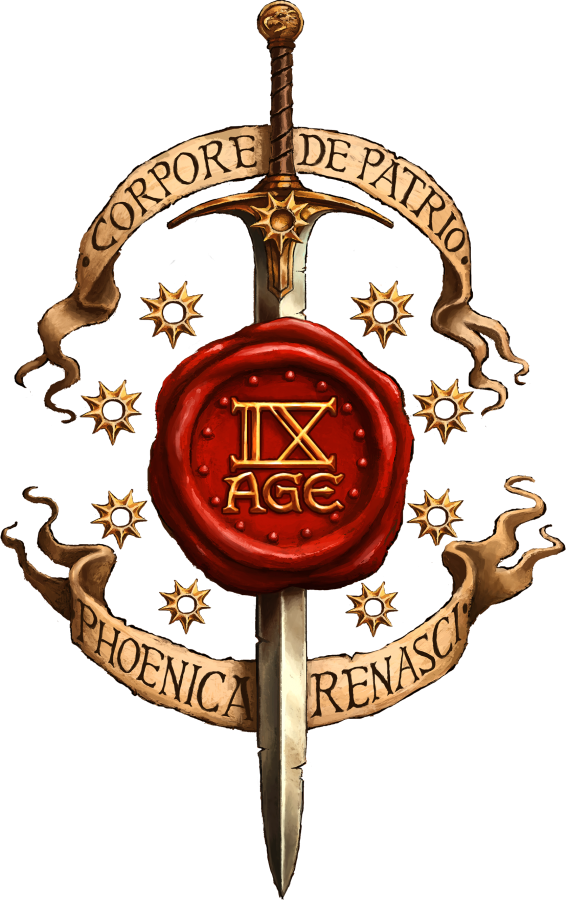
\includegraphics[height=10cm]{../Layout/pics/logo_9th.png}%
}

\vspace*{-1cm}
{\antiquefont\fontsize{50}{60}\selectfont \booktitle
\vspace{0.4cm}

\fontsize{14}{16.8}\selectfont \labels@armyrules{}

Beta v\version{} - \today{}}

\ifdef{\frenchversion}{{\fontsize{14}{16.8}\selectfont \vspace{0.2cm}\noindent\texttt{VF \frenchversion}}}{}
\vfill

\begin{tabular}{@{}m{2cm}@{\hskip 20pt}m{13cm}@{}}
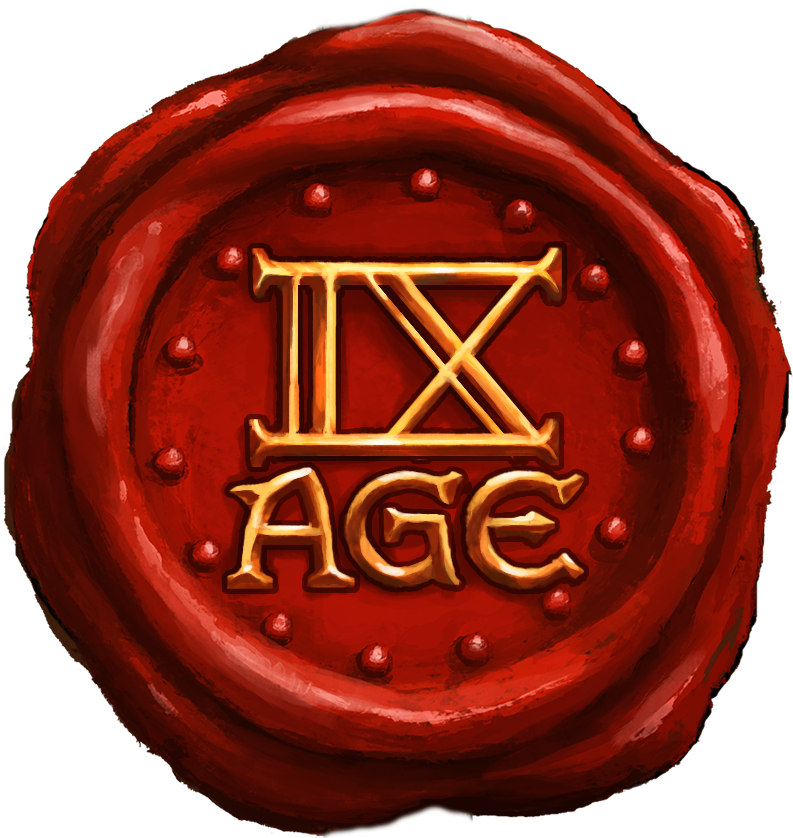
\includegraphics[width=2cm]{../Layout/pics/seal_9th.png} &
{\fontsize{10}{12}\selectfont \textcolor{black!50}{\noindent\labels@frontpagecredits}}

\ifdef{\frontpageaddstuff}{{\fontsize{10}{12}\selectfont \noindent\textcolor{black!50}{\frontpageaddstuff}}}{}

\vspace*{10pt}
\noindent{\fontsize{10}{12}\selectfont \textcolor{black!50}{\labels@license}}
\tabularnewline
\end{tabular}


\end{center}

\newpage

\thispagestyle{empty}

{\fontsize{10}{12}\selectfont

\ifdef{\labels@introduction}{\labels@introduction}{\vphantom{1pt}}
\vfill

\noindent\newrule{\labels@rulechanges}

\bigskip
\noindent \labels@latexcredit
}


\end{titlepage}

\restoregeometry

\startarmywiderules

\armywideruleentry{\invocation}

Les profils d'unité contiennent une catégorie appelée \invocation{} qui donne le nombre de Points de Vie Ressuscités grâce à l'\necromancysignature{} et la \necromancyspellfour{} de la Discipline \necromancy{}.

\armywideruleentry{\masterofundeath}

Un Personnage doit être le \textbf{\master{}} de l'armée. Au début de la partie, le Général est toujours le \master{}.

\closearmywiderules

\vspace*{1.5cm}
\startarmyspecialrules

\armyspecialruleentry{\ashestoashes}

À la fin de n'importe quelle phase durant laquelle le \master{} est retiré du jeu en tant que perte, toute unité de l'armée qui possède au moins une figurine avec la règle \ashestoashes{} doit faire un test de Commandement. Si le test échoue, l'unité subit un nombre de blessures équivalent à la différence entre le résultat obtenu et la valeur de Commandement du test, sans aucune sauvegarde autorisée. Ces blessures sont réparties comme pour la règle \unstable{}, mais ne peuvent pas être assignées à une figurine n'ayant pas la règle \ashestoashes{}. Le montant de blessures est réduit de un si l'unité est à portée de \holdyourground{}.

\vspace*{5pt}À la fin du Tour de Joueur suivant la mort du \master{}, un nouveau \master{} peut être choisi. Pour ce faire, vous devez nommer un autre Personnage éligible, c'est à dire un \wizard{} utilisant la Discipline \necromancy{}. Ce Personnage est le nouveau \master{}.

\vspace*{5pt}Au début de chacun de vos Tours de Joueur sans nouveau \master{}, toute unité qui possède au moins une figurine avec la règle \ashestoashes{} doit faire un nouveau test de Commandement, et subir des blessures comme décrit ci-dessus.

\armyspecialruleentry{\wailofwoe}

L'élément de figurine dispose des Attaques Spéciale de Tir et de Corps à Corps suivantes :
\begin{itemize}[label={-}]
\item Attaque Spéciale de Tir, normalement utilisée pendant la Phase de Tir, même après une Marche Forcée. Choisissez une cible en utilisant les règles habituelles des Attaques de Tir. L'attaque touche automatiquement avec le profil suivant :\newline
\range{8}, Force 4, \magicalattacks{}, \multipleshots{1D6+2}.
\item Attaque Spéciale de Corps à Corps, normalement utilisée pendant la Phase de Corps à Corps. L'élément de figurine peut remplacer ses attaques non spéciales par celle-ci, qui se fait à son Initiative. Ciblez une unité au contact socle à socle : elle subit 1D3+1 touches de Force 4 avec la règle \magicalattacks{}.
\end{itemize}


\armyspecialruleentry{\awaken{X}}

La figurine peut Ressusciter des PVs au-delà de l'effectif de départ de toutes les unités mentionnées entre parenthèses, en suivant les modalités de la règle \raisewounds{}. L'effectif de départ est le nombre de figurines choisi sur la liste d'armée. La taille des unités ne peut cependant pas être augmentée au delà du double de l'effectif de départ.

\newpage
\armyspecialruleentry{\reaper}

Une unité composée uniquement de figurines possédant cette règle peut ignorer les décors et unités entre points de départ et d'arrivée durant l'étape des Autres Mouvements, mais doit respecter la règle des \distance{1} à la fin du déplacement. L'unité peut effectuer une \sweepingattack{}. L'ennemi subit une touche par figurine possédant la règle \reaper{} ayant traversé la cible. Ces touches utilisent la Force, les règles spéciales et les bonus d'arme affectant normalement les Attaques de Corps à Corps des figurines, comme \flamingattacks{} ou \armourpiercing{}.

\armyspecialruleentry{\vampiric{X}}

Une unité composée uniquement de figurines avec cette règle peut effectuer des Marches Forcées même lorsqu'elle se trouve hors de portée de la règle \inspiringpresence{} du Général. Elle doit toujours effectuer un test de Commandement si elle se trouve dans un rayon de \distance{8} d'une unité ennemie.

\vspace*{5pt}À la fin de chaque Phase de Corps à Corps, les unités avec cette règle peuvent faire des jets pour la règle \vampiric{}. Lancez 1D6 pour chaque Personnage \vampiric{} qui a infligé au moins une blessure non sauvegardée durant cette Phase de Corps à Corps, et 1D6 si au moins une figurine ordinaire \vampiric{} de l'unité l'a fait. Un jet \vampiric{} est réussi si le résultat du dé est de X ou plus, où X est le nombre entre parenthèses. Un résultat de \result{1} est toujours un échec, tandis qu'un \result{6} est toujours un succès. Les figurines avec la règle \largetarget{} ont un malus de -2 sur le résultat des dés de leur jet \vampiric{}, jusqu'à un minimum de 1. Un Personnage qui réussit un jet \vampiric{} Récupère un Point de Vie. Une unité qui a réussi un jet \vampiric{} provenant de ses figurines ordinaires Ressuscite un unique PV dans l'unité.

\armyspecialruleentry{\necromanticaura}

Toutes les unités amies dans un rayon de \distance{6} d'une ou plusieurs figurines avec cette règle réduisent le nombre de blessures qu'elle subissent par les règles \ashestoashes{} et \unstable{} de 1. Les figurines avec la règle \necromanticaura{} ne peuvent pas en bénéficier elles-mêmes.


\closearmyspecialrules







\newpage
\toctarget{bloodlinestitle}{\startarmynewsection{Dynasties Vampiriques}}

\spaceaftersection{}

Une armée des Conclaves Vampiriques peut choisir de représenter une unique Dynastie Vampirique. Dans ce cas, tous les \vampirelords{} et \vampireheroes{} de l'armée doivent prendre l'amélioration correspondant à la Dynastie. À moins que le contraire ne soit précisé, toutes les règles associées à un Vampire ne s'appliquent qu'à l'élément de figurine prenant l'amélioration et pas aux montures.

\armynewsubsection{Pouvoir Dynastique Ancien}

Les \vampirelords{} appartenant à une \bloodline{} peuvent accéder au \ancientbloodpower{} de leur \bloodline{} plutôt que de prendre un \bloodpower{}. Chaque \ancientbloodpower{} est \oneofakind{}.

\armynewsubsection{\bloodties{X}}

Certaines troupes du Livre d'Armée sont notées comme étant des \bloodties{}, suivies entre parenthèses de la \bloodline{} à laquelle elles appartiennent. Si la \bloodline{} des Personnages \vampires{} de l'armée correspond à celle entre parenthèses, vous pouvez prendre l'option décrite à la suite.

\armynewsubsection{\brotherhood{}\dotfill\pts{30/10}}

\begin{wrapfigure}[5]{L}{0cm}
\centering
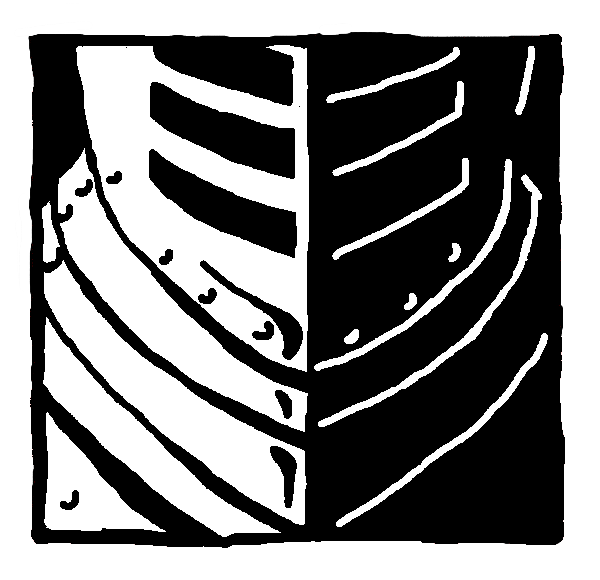
\includegraphics[width=\logosize]{pics/logo_brotherhood.png}
\end{wrapfigure}
Le Vampire gagne +2 en Capacité de Combat et porte une \platearmour{}. Il ne peut prendre qu'un seul Niveau de Magie supplémentaire et ne peut utiliser que la Discipline \necromancy{}. Il ne peut jamais refuser de Défi et doit en lancer dès qu'il le peut, à moins qu'une autre figurine ne le fasse en premier.

\vspace{0.5cm}
\bloodtie{} : \textbf{\vampireknights}.

\vspace{0.5cm}
\ancientbloodpower{} : \textbf{\crimsonrage}\dotfill\pts{65}\newline%
Chaque blessure non sauvegardée infligée par des attaques normales du Vampire, avant d'appliquer les \multiplewounds{}{}, déclenche une nouvelle attaque à la même Initiative. Résolvez ces attaques avant de retirer les pertes. Ces attaques additionnelles ne génèrent pas d'autres attaques.

\armynewsubsection{\bloodline{} \vonkarnstein{}\dotfill\pts{25/10}}

\begin{wrapfigure}[5]{R}{0cm}
\centering

\includegraphics[width=\logosize]{pics/logo_vonkarnstein.png}
\end{wrapfigure}
Le vampire peut relancer ses jets ratés pour la règle \vampiric{}. La présence d'un ou plusieurs Vampires \vonkarnstein{} dans un corps à corps octroie un bonus de +1 au Résultat de Combat de leur camp. Une unité avec la règle \undead{} rejointe par un Vampire \vonkarnstein{} peut effectuer une Marche Forcée comme si elle avait la règle \vampiric{}. La portée des éventuelles règles \inspiringpresence{} et \holdyourground{} du Vampire est augmentée de \distance{6}. 

\vspace{0.5cm}
\bloodties{} : \textbf{\darkcoach}.

\vspace{0.5cm}
\ancientbloodpower{} : \textbf{\stormcaller}\dotfill\pts{65}\newline%
Le Vampire possède un \boundspell{4} : \heavensspelltwo{} (Discipline \heavens{}). Toutes les unités dans un rayon de \distance{12} gagnent la règle \hardtarget{}. De plus, une fois par partie, le Vampire peut donner à toutes les figurines ordinaires de son unité et lui-même les règles \lightningattacks{} et \lightningreflexes{}. Cette capacité doit être activée au début d'une Manche de Corps à Corps et dure jusqu'à la fin de cette Manche.

\newpage
\armynewsubsection{\bloodline{} \lamia{}\dotfill\pts{40/25}}

\begin{wrapfigure}[7]{L}{0cm}
\centering

\includegraphics[width=\logosize]{pics/logo_lamia.png}
\end{wrapfigure}
La Vampire perd une Attaque et obtient la règle \lightningreflexes{}. Si elle ne porte aucune Armure, sans compter la \mountsprotection{} et la \innatedefence{}, elle obtient également la règle \distracting{}. Les Défis lancés par la Vampire doivent être acceptés si possible et les figurines en Défi contre une \lamia{} doivent réussir un test de Commandement avec un malus additionnel de -1. Dans le cas d'un échec, elles doivent relancer leurs jets pour toucher réussis pendant cette Manche de Corps à Corps. La Vampire n'a accès qu'aux Disciplines \light{}, \shadows{} ou \necromancy{}.

\vspace{0.5cm}
\bloodties{} : \textbf{\courtofthedamned}.

\vspace{0.5cm}
\ancientbloodpower{} : \textbf{\commandment}\dotfill\pts{50}\newline%
Toutes les figurines ordinaires de l'unité rejointe par la Vampire obtiennent une Capacité de Combat de 5.

\armynewsubsection{\bloodline{} des \strigois{}\dotfill\pts{55/30}}

\begin{wrapfigure}[5]{R}{0cm}
\centering
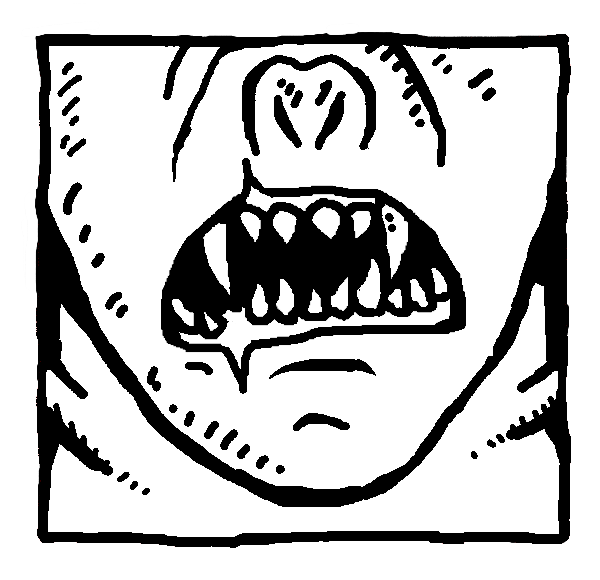
\includegraphics[width=\logosize]{pics/logo_strigoi.png}
\end{wrapfigure}
Le Vampire et sa monture obtiennent les règles \regeneration{5} et \hatred{}. Le Vampire gagne +1 Point de Vie, ne peut pas prendre de monture à l'exception d'une \shriekinghorror{} et ne peut porter aucune Armure. Il ne peut acheter qu'un seul Niveau de Magie supplémentaire et doit utiliser la Discipline \wilderness{} ou \necromancy{}.

\vspace{0.5cm}
\bloodties{} : \textbf{\ghouls{}}.

\vspace{0.5cm}
\ancientbloodpower{} : \textbf{\bestialbulk}\dotfill\pts{55}\newline%
Figurines à pied uniquement.

\vspace{5pt}\noindent{}Le type de troupe du Vampire devient \monstrousinfantry{} et la taille de son socle passe à \unit{40x40}{\milli\meter}. Il gagne +1 PV, est équipé d'une \pw{} et ne peut manier aucune autre Arme, standard ou magique.

\armynewsubsection{\bloodline{} \nosferatu{}\dotfill\pts{110/50}}

\begin{wrapfigure}[7]{L}{0cm}
\centering
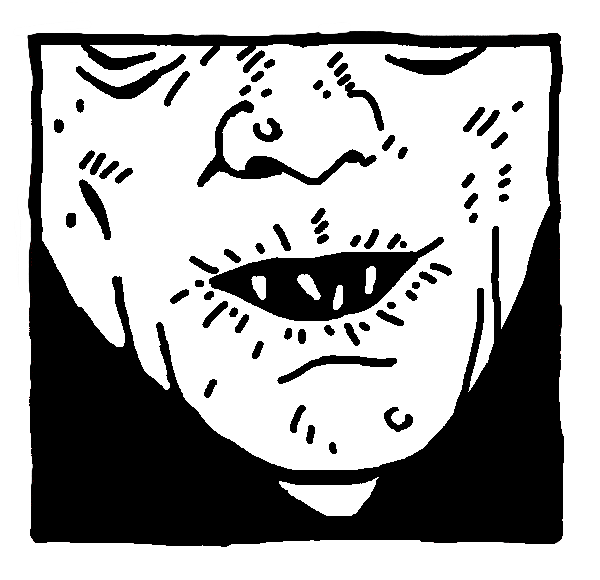
\includegraphics[width=\logosize]{pics/logo_nosferatu.png}
\end{wrapfigure}
Le Vampire perd une Attaque, subit un malus de -2 en Capacité de Combat et ne peut porter aucune Armure, à l'exception de la \mountsprotection{} et de la \innatedefence{}. Il ne peut pas porter d'Arme standard. Il devient un \magiclevel{2} si c'est un Héros ou un \magiclevel{4} si c'est un Seigneur. Il gagne la règle \awaken{\skeletons{}, \zombies{}} et génère un sort supplémentaire, mais doit échanger un de ses sorts pour l'\necromancysignature{} (Discipline \necromancy{}).

\vspace{0.5cm}
\bloodties{} : \textbf{\wraiths}.

\vspace{0.5cm}
\ancientbloodpower{} : \textbf{\bloodmagic}\dotfill\pts{75}\newline%
Le Vampire compte toujours comme ayant utilisé un Dé de Pouvoir de moins en cas de Fiasco. Immédiatement après avoir lancé les dés pour déterminer les Flux Magiques pendant votre tour, vous pouvez choisir de relancer un des dés. Dans ce cas, le Vampire subit une blessure sans aucune sauvegarde possible à la fin de la Phase de Magie.

\closearmynewsection








\newpage
\toctarget{bloodlinepowerstitle}{\startarmynewsection{Pouvoirs Dynastiques}}

\spaceaftersection{}

Les \vampirelords{} et les \vampireheroes{} peuvent acheter une unique amélioration appelée Pouvoir Dynastique Vampirique. Dans le cas d'une armée Indépendante, c'est à dire sans Dynastie, tous les Pouvoirs Dynastiques sont de type \oneofakind{}. Si votre armée représente une Dynastie, seuls les Pouvoirs de cette Dynastie peuvent être pris par vos Vampires, mais ils peuvent être dupliqués.

\begin{multicols}{2}\raggedcolumns

\begin{center}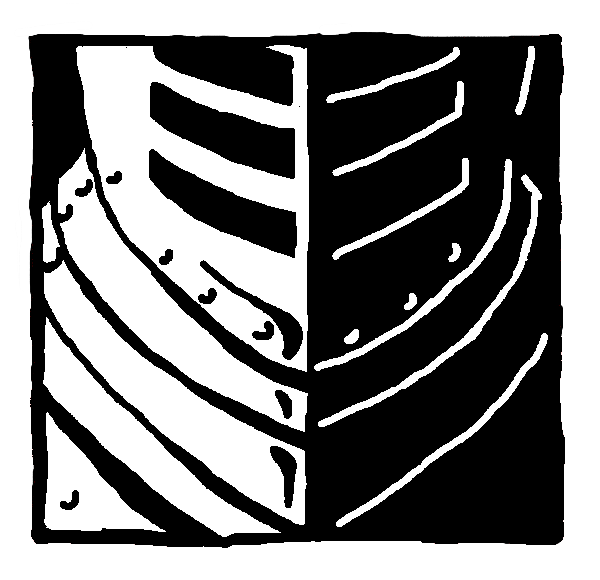
\includegraphics[width=2cm]{pics/logo_brotherhood.png}\end{center}
\vspace*{-1.5cm}
\armynewsubsection{\begin{center}Indépendant ou \brotherhood{}\end{center}}

\vspace*{-0.2cm}
\startpricelist

\pricelistitem{\perfectwarrior}{35} Le Vampire gagne les règles \weaponmaster{} et \lethalstrike{}. Il est équipé d'un \shield{}, d'une \gw{}, d'une \halberd{}, d'une \lance{} et d'une \pw{}.

\pricelistitem{\eternalduelist}{30} Lorsqu'il combat en défi, le Vampire peut relancer ses jets pour toucher et pour blesser ratés.

\endpricelist

\begin{center}
\includegraphics[width=2cm]{pics/logo_vonkarnstein.png}\end{center}
\vspace*{-1.5cm}
\armynewsubsection{\begin{center}Indépendant ou \vonkarnstein{}\end{center}}

\vspace*{-0.2cm}
\startpricelist

\pricelistitem{\refinedtaste}{25} Le Vampire gagne la règle \vampiric{2}.

\pricelistitem{\hourofthewolf}{20} Le Vampire gagne la règle \awaken{\zombies{}, \direwolves{}, \batswarms{}, \greatbats{}}. Le Vampire ainsi que les figurines de l'unité qu'il rejoint gagnent la règle \swiftstride{}, à l'exception des autres Personnages ayant la règle \vampiric{}.

\endpricelist

\begin{center}
\includegraphics[width=2cm]{pics/logo_lamia.png}\end{center}
\vspace*{-1.5cm}
\armynewsubsection{\begin{center}Indépendant ou \lamia{}\end{center}}

\vspace*{-0.2cm}
\startpricelist

\pricelistitem{\mesmerizinggaze}{35} Le Vampire possède un \boundspell{4}. \lustspellfour{} (Discipline \lust{}).

\pricelistitem{\maskofinnocence}{25} Les unités au contact d'un ou plusieurs Vampires avec ce pouvoir subissent un malus de -1 en Commandement.

\endpricelist
\columnbreak

\begin{center}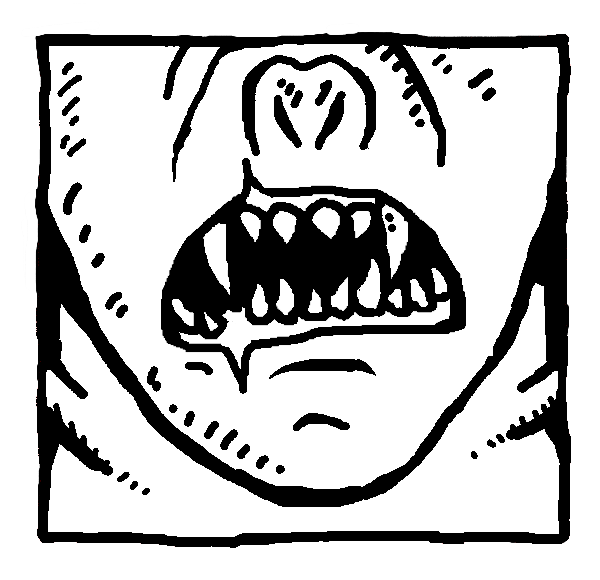
\includegraphics[width=2cm]{pics/logo_strigoi.png}\end{center}
\vspace*{-1.5cm}
\armynewsubsection{\begin{center}Indépendant ou \strigoi{}\end{center}}

\vspace*{-0.2cm}
\startpricelist

\pricelistitem{\curseoftheblood}{70} Le Vampire gagne la règle \regeneration{5}. S'il possédait déjà une \regeneration{}, il gagne \regeneration{4}. Toutes les \ghouls{} dans la même unité que le Vampire ainsi que son éventuelle monture gagnent la règle \regeneration{6}. Si une figurine affectée par cette capacité possède déjà la \regeneration{}, sa sauvegarde de \regeneration{} est améliorée d'un point, pour obtenir 4+ au mieux.

\pricelistitem{\ghoullord}{55} Le Vampire et sa monture gagnent les règles \poisonedattacks{} et \armourpiercing{1}. Les \ghouls{} de l'unité qu'il rejoint gagnent la règle \hatred{}.

\endpricelist

\begin{center}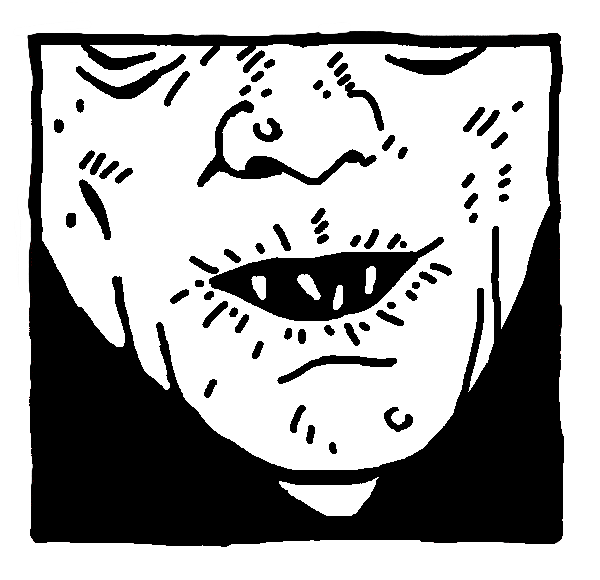
\includegraphics[width=2cm]{pics/logo_nosferatu.png}\end{center}
\vspace*{-1.5cm}
\armynewsubsection{\begin{center}Indépendant ou \nosferatu{}\end{center}}

\vspace*{-0.2cm}
\startpricelist

\pricelistitem{\arcaneknowledge}{30} Les sorts lancés par le Vampire ont une Portée augmentée de \distance{6}. Cet effet est réduit à \distance{3} pour les sorts de type Aura. Les sorts de Vortex, les \boundspells{} et les sorts sans Portée ne sont pas affectés.

\pricelistitem{\forbiddenpath}{20} Le Vampire peut générer ses sorts dans la Discipline \necromancy{} ou dans n'importe laquelle des Disciplines Communes, à l'exception \nature{}.

\endpricelist

\vspace*{\fill}
\end{multicols}

\closearmynewsection









\startarmymagicalitems

\armymagicalweapons

\startpricelist

\pricelistitem{\bladeofredthirst}{40} Vampires uniquement.

Type: \hw{}. Le Vampire maniant cette lame gagne la règle \vampiric{3}. L'élément de figurine lance 1D6 pour chaque blessure qu'il inflige dans le cadre de sa règle \vampiric{}, au lieu d'un seul dé. Chaque jet \vampiric{} réussi lui rend un PV, puis tout excès de PV ainsi Ressuscité peut être utilisé pour \raisewounds{} dans l'unité que le personnage a rejointe.

\endpricelist

\armymagicalarmour

\startpricelist

\pricelistitem{\redplateofgillesderaux}{40} Type : \platearmour{}. Le porteur gagne +1 Point de Vie.

\endpricelist

\armytalismans

\startpricelist

\pricelistitem{\eternalring}{60/50} Vampires uniquement.

Le porteur possède une \wardsave{2} contre la première blessure subie de la partie, après les Sauvegardes d'Armure. Il est immunisé aux effets des règles \lethalstrike{} et \multiplewounds{}{}.

\pricelistitem{\mantleofnight}{40} Infanterie ou Cavalerie uniquement.

Toute figurine allouant des attaques de Corps à Corps au porteur ne reçoit aucun bonus de type +X en Force lié à ses Armes, qu'elles soient magiques ou standard.

\endpricelist

\armyenchanteditems

\startpricelist

\pricelistitem{\tulliusteeth}{50} Le porteur gagne la règle \distracting{}. Toutes les figurines ordinaires d'\infantry{} et de \cavalry{} de son unité gagnent la règle \parry{}.

\endpricelist

\armyarcaneitems

\startpricelist

\pricelistitem{\staffofgerhardtheblack}{45} Une armée possédant cet objet peut relancer ses jets de Canalisation ratés. De plus, quand le porteur lance le sort \necromancysignature{} (Discipline \necromancy{}), un dé pour déterminer le nombre de Points de Vie Ressuscités peut être relancé pour chaque unité ciblée.

\pricelistitem{\unholytome}{35} \boundspell{4}. \necromancyspelltwo{} (Discipline \necromancy{}).

\pricelistitem{\eyeofsetesh}{15} Une seule utilisation. À la fin d'une Phase de Magie adverse, vous pouvez mettre un Dé de Dissipation inutilisé de côté. Ce dé pourra être ajouté à votre réserve comme Dé de Pouvoir, juste après avoir déterminé les Flux de Magie.

\endpricelist

\armymagicalbanners

\startpricelist

\pricelistitem{\blackstandardofzagvozd}{40} Toutes les figurines de l'unité obtiennent une \wardsave{4} contre les Attaques de Tir. 

\pricelistitem{\bannerofthebarrowskings}{25} Les figurines de \barrowknights{} et de \barrowguards{} de l'unité obtiennent +1 pour toucher au Corps à Corps.

\endpricelist

\closearmymagicalitems









%%% START OF THE ARMYLIST - Translators shouldn't have to edit it %%%


%%% v0.10.1

\armylist

\lordstitle

\showunit{
	name={\vampirelord},
	cost={\newrule{205}},
	profile={ < 6 7 5 5 5 3 7 5 10},
	type=\infantry ,
	basesize=20x20,
	unitsize=1,
	commontype=\vampiriccommonrules ,
	commonspecialrules={\undead,\fear,\vampiric{6}},
	specialrules={\awaken{\zombies},\masterofundeath},
	magiclevel=1,
	magicpaths={\necromancy, \shadows, \death},
	options={
		\magiclevelchoice{
			\magiclevel{2}=\newrule{25},
			\magiclevel{3}=\newrule{95},
		},
		\magicalitemsallowance = \upto < 100,
		\bloodlinechoice = \unlimited,
		\bloodpowerchoice = \unlimited,
		\Maytakea{} \shield =5,
		\armouronechoice{
			\la =5,
			\ha =10,
		},
		\weapononechoice{
			\ahw =\newrule{10},
			\halberd =\newrule{15},
			\gw =\newrule{20},
			\lance =20,
		}
	},
	mounts={\skeletalsteed =20, \monstrousrevenant =100, \courtofthedamned{} \only{\lamia}=190, \shriekinghorror{} \only{\strigoi}=200, \zombiedragon =\newrule{270}}
}

\showunit{
	name={\necromancerlord},
	cost={\newrule{175}},
	profile={ < 4 3 3 3 4 3 3 1 8},
	type= \infantry ,
	basesize=20x20,
	unitsize=1,
	commontype=\undeadcommonrules ,
	commonspecialrules={\undead},
	specialrules={\awaken{\zombies , \skeletons}, \masterofundeath},
	magiclevel=3,
	magicpaths={\necromancy, \fire, \death},
	options={
		\magiclevel{4}=\newrule{35},
		\magicalitemsallowance = \upto < 100,
	},
	mounts={\skeletalsteed =20, \monstrousrevenant =100, \cadaverwagon =100}
}

\heroestitle


\showunit {
	name={\vampirehero},
	cost=80,
	profile={ < 6 6 4 5 4 2 6 4 8},
	type=\infantry ,
	basesize=20x20,
	unitsize=1,
	commontype=\vampiriccommonrules ,
	commonspecialrules={\undead,\fear,\vampiric{6}},
	specialrules={\awaken{\zombies}, \masterofundeath},
	magicpaths={\necromancy, \shadows, \death},
	options={
		\bsboption{} \notif{\strigoi}= 25,
		\magiclevelchoice{
			\magiclevel{1}=\newrule{40},
			\magiclevel{2}=\newrule{65},
		},
		\magicalitemsallowance = \upto < 50,
		\bloodlinechoice =\unlimited,
		\bloodpowerchoice =\unlimited,		
		\Maytakea{} \shield =5,
		\armouronechoice{
			\la =5,
			\ha =10,
		},
		\weapononechoice{
			\ahw =5,
			\halberd =\newrule{10},
			\gw =10,
			\lance =15,
		}
	},
	mounts={\skeletalsteed =20, \monstrousrevenant =120}
}


\showunit{
	name={\necromancer},
	cost={\newrule{65}},
	profile={ < 4 3 3 3 3 2 3 1 7},
	type= \infantry ,
	basesize=20x20,
	unitsize=1,
	commontype=\undeadcommonrules ,
	commonspecialrules={\undead},
	specialrules={\awaken{\zombies, \skeletons}, \masterofundeath},
	magiclevel=1,
	magicpaths={\necromancy, \fire, \death},
	options={
		\magiclevel{2}=\newrule{25},
		\magicalitemsallowance = \upto < 50,
	},
	mounts={\skeletalsteed = 20, \cadaverwagon = 100}
}

\showunit{
	name={\barrowking},
	cost=80,
	profile={ < 4 4 - 4 5 3 4 3 9},
	type=\infantry ,
	basesize=20x20,
	unitsize=1,
	commontype=\undeadcommonrules ,
	commonspecialrules={\undead, \newrule{\ashestoashes}},
	specialrules={\multiplewounds{2}{\infantry, \cavalry, \warbeasts}, \lethalstrike, \notaleader, \magicalattacks},
	equipment={\ha, \shield},
	options={
		\bsboption = 25,
		\magicalitemsallowance = \upto < 50,
		\weapononechoice{
			\ahw =\newrule{3},
			\halberd =\newrule{4},
			\lance =\newrule{6},
			\gw =\newrule{6},
		},
		\maybeupgradedto{} \unlivingshield = 15
	},
	mounts={\skeletalsteed = 20},
	unitrules={
		\unitrule{\unlivingshield}{\unlivingshieldrule}
	}
}

\showunit {
	name={\fellwraith},
	cost=\newrule{55},
	profile={\fellwraith < 6 3 - 3 3 2 2 3 5,
		     \banshee < 6 3 - 3 3 2 3 1 5
	},
	type=\infantry ,
	basesize=20x20,
	unitsize=1,
	commontype=\undeadcommonrules ,
	commonspecialrules={\undead, \ashestoashes},
	specialrules={\ethereal, \reaper, \notaleader, \terror},
	options={
		\mustbecomeoneofthefollowing{
			\fellwraith = \free,
			\banshee = 30
		}
	},
	additional={%
		\setlength{\columnseprule}{1pt}
		\renewcommand{\columnseprulecolor}{\color{black!30}}
		\begin{multicols}{2}
		\begin{center} \LARGE\antiquefont\fellwraith{} \end{center}%
		
		\def\tempspecialrules{\armourpiercing{6}}%
		\specialrules{\tempspecialrules}

		\def\tempoptions{%
			\newrule{\Maytakea{} \gw{}} = 10,
			\newrule{\magicalweaponallowance} = \upto < 50,		
		}%
		\vspace*{0.15cm}\options{\tempoptions}

		\def\tempmounts{\skeletalsteed{} \newrule{\wordwith{} \freereform{}} = 20}%	
		\mounts{\tempmounts}
			
		\columnbreak
		\begin{center} \LARGE\antiquefont\banshee{} \end{center}

		\def\tempspecialrules{\chillingshriek{2, 8}}%
		\specialrules{\tempspecialrules}%
		\end{multicols}
		\setlength{\columnseprule}{0pt}
	},
}


\coreunitstitle

\showunit{
	name={\zombies},
	cost=60,
	profile={ < 4 1 0 3 3 1 1 1 2},
	invocation={2D6+3},
	type=\infantry ,
	basesize=20x20,
	unitsize=20,
	maxmodels=60,
	costpermodel=3,
	commontype=\undeadcommonrules ,
	commonspecialrules={\undead, \ashestoashes},
	commandgroup={musician=10, banner=10}
}

\showunit{
	name={\skeletons},
	cost=40,
	profile={< 4 2 2 3 3 1 2 1 6},
	invocation={1D6+3},
	type=\infantry ,
	basesize=20x20,
	unitsize=10,
	maxmodels=60,
	costpermodel=4,
	commontype=\undeadcommonrules ,
	commonspecialrules={\undead, \ashestoashes},
	equipment={\la},
	options={
		\spear = \free,
		\shield = \permodel < 1
	},
	commandgroup={champion=10, musician=10, banner=10, veteranstandardbearer=*},
	additional={%
		* \veteranstandardbearernote
	}
}

\showunit{
	name={\ghouls},
	cost=90,
	profile={< 4 3 - 3 4 1 3 2 6},
	invocation={1D6+3},
	type= \infantry ,
	basesize=20x20,
	unitsize=10,
	maxmodels=40,
	costpermodel=9,
	commontype=\undeadcommonrules ,
	commonspecialrules={\undead, \ashestoashes},
	specialrules={\poisonedattacks},
	options={
		\skirmishers{} \ifNmodelsorless{15}= \permodel < 1,
		\bloodties{\strigoi}\spacebeforecolon{}:\newline\vanguard{}*= \permodel < 2,
	},
	commandgroup={champion=10, musician=\newrule{10}, banner=\newrule{10}, veteranstandardbearer =yessir},
	additional={%
		* \strigoivanguardnote
	}
}

\showunit{
	name={\direwolves},
	cost=40,
	profile={
		< 9 3 0 3 3 1 3 1 3},
	invocation={1D3+3},
	type=\warbeast ,
	basesize=25x50,
	unitsize=5,
	maxmodels=15,
	costpermodel=7,
	commontype=\undeadcommonrules ,
	commonspecialrules={\undead, \ashestoashes},
	specialrules={\vanguard, \thunderouscharge},
	commandgroup={champion=10}
}

\showunit{
	name={\batswarm},
	cost=60,
	profile={
		< 1 2 - 2 2 4 3 4 3},
	invocation={1D6+3},
	type=\swarm ,
	basesize=40x40,
	unitsize=2,
	maxmodels=10,
	costpermodel=15,
	commontype=\undeadcommonrules ,
	commonspecialrules={\undead, \ashestoashes},
	specialrules={\fly{6}},
	unitrules={
		\unitrule{\stormofwings}{\stormofwingsrule}
	}
}

\specialunitstitle

\showunit{
	name={\barrowknights},
	cost=120,
	profile={\knight < 4 3 - 4 4 1 3 1 \newrule{7},
			 \steed < 8 2 - 3 3 1 2 1 3
	},
	invocation= 2 ,
	type=\cavalry ,
	basesize=25x50,
	unitsize=5,
	maxmodels=15,
	costpermodel=24,
	commontype=\undeadcommonrules ,
	commonspecialrules={\undead, \ashestoashes},
	specialrules={\magicalattacks, \multiplewounds{2}{\infantry , \cavalry , \warbeasts}, \lethalstrike{} \only{\knight}, \ethereal{} \only{\steed}},
	equipment={\ha , \shield , \lance , \mountsprotection{5}},
	commandgroup={champion=10, musician=10, banner=10, bannerallowance=50}
}

\showunit{
	name={\barrowguards},
	cost=100,
	profile={
		< 4 3 - 4 4 1 3 1 \newrule{7}},
	invocation= 1D3+3 ,
	type=\infantry,
	basesize=20x20,
	unitsize=10,
	maxmodels=40,
	costpermodel=10,
	commontype=\undeadcommonrules ,
	commonspecialrules={\undead, \ashestoashes},
	specialrules={\magicalattacks, \multiplewounds{2}{\infantry , \cavalry , \warbeasts},\lethalstrike, \bodyguard{\general, \barrowking}},
	equipment={\ha},
	options={
		\maytakeoneofthefollowing{
			\halberd = \permodel < 2,
			\gw = \permodel < 2,
			\shield = \permodel < 1,
		},
	},
	commandgroup={champion=10, musician=10, banner=10, bannerallowance=50}
}

\showunit{
	name={\ghasts},
	cost=110,
	profile={< 6 3 - 4 5 3 2 3 5},
	invocation= 2 ,
	type=\monstrousinfantry ,
	basesize=40x40,
	unitsize=3,
	maxmodels=10,
	costpermodel=48,
	commontype=\undeadcommonrules ,
	commonspecialrules={\undead, \ashestoashes},
	specialrules={\poisonedattacks, \fear,  \regeneration{5}},
	commandgroup={champion=10}
}

\showunit{
	name={\vampirespawn},
	cost=\newrule{117},
	profile={
		< 6 4 - 5 4 3 4 3 8},
	invocation= 2 ,
	type=\monstrousinfantry ,
	basesize=40x40,
	unitsize=3,
	maxmodels=\newrule{6},
	costpermodel=\newrule{39},
	commontype=\vampiriccommonrules ,
	commonspecialrules={\undead, \vampiric{6}, \fear},
	specialrules={\frenzy, \fly{9}},
	commandgroup={champion=10},
	options={
		\newrule{\vampirespawnskirmishersoption} = \permodel < 3,
	}
}

\showunit{
	name={\phantomhost},
	cost=70,
	profile={< 6 3 - 3 3 4 1 4 4},
	invocation= 1D3+3 ,
	type=\infantry,
	basesize=40x40,
	unitsize=2,
	maxmodels=6,
	costpermodel=\newrule{30},
	commontype=\undeadcommonrules ,
	commonspecialrules={\undead, \ashestoashes},
	specialrules={\ethereal, \fear}
}

\showunit{
	name={\greatbats},
	cost=40,
	profile={
		< 1 3 - 3 3 2 3 2 3},
	invocation= 1D3+3 ,
	type=\warbeast ,
	basesize=40x40,
	unitsize=2,
	maxmodels=9,
	costpermodel=14,
	commontype=\undeadcommonrules ,
	commonspecialrules={\undead, \ashestoashes},
	specialrules={\skirmishers, \fly{10}},
}

\showunit{
	name={\varkolak},
	cost=\newrule{165},
	profile={
		< 8 5 - 6 5 4 4 5 7},
	invocation= 1 ,
	type=\monstrousbeast ,
	basesize=50x50,
	unitsize=1,
	commontype=\vampiriccommonrules ,
	commonspecialrules={\undead, \vampiric{3}, \fear},
	specialrules={\hatred, \regeneration{4}},
	options={
		\maytakeoneofthefollowing{
			\vanguard{}= 20,
			\stomp{1D3+1}= 20,
			\fly{8}= 40,
		}
	}
}

\showunit{
	name={\cadaverwagon},
	cost=80,
	profile={
		\cadaverwagon < - - - 4 4 4 - - -,
   		\cadavermaster < - 3 - 3 - -  3 1 5,
		\shamblinghorde < 4 1 - 3 3 -  1 * -	
	},
	invocation= 1 ,
	type=\chariot ,
	basesize=50x100,
	unitsize=1,
	commontype=\undeadcommonrules ,
	commonspecialrules={\undead, \ashestoashes},
	specialrules={\randomattacks{2D6} \only{\shamblinghorde}, \wakethedead, \cart, \regeneration{4}},
	equipment={\mountsprotection{5}},
	options={
		\endlesshorde = 25,
		\maytakeoneofthefollowing{
			\bonepyre = 10,
			\bringoutyourdead = 15,
			\necromanticaura = 20
		}
	},
	unitrules={
		\unitrule{\cart}{\cartrule}
		\unitrule{\endlesshorde}{\endlesshorderule}
		\unitrule{\bonepyre}{\bonepyrerule}
		\unitrule{\bringoutyourdead}{\bringoutyourdeadrule}
	}
}

\rareunitstitle


\showunit{
	name={\vampireknights},
	cost=225,
	profile={
		\knight < 4 5 3 5 4 2 5 2 8,
		\undeadmount < 8 3 0 4 3 1 2 1 3
	},
	invocation= 2 ,
	type=\cavalry ,
	basesize=25x50,
	unitsize=5,
	maxmodels=\newrule{8},
	costpermodel=45,
	commontype=\vampiriccommonrules ,
	commonspecialrules={\undead,\fear,\vampiric{6}},
	equipment={\lance , \ha , \shield , \mountsprotection{6}, \barding},
	options={
		\bloodties{\brotherhood}\spacebeforecolon{}:\newline\vampireknightbloodtiesoption{}= \permodel < 15,
	},
	commandgroup={champion=10, musician=10, banner=10, bannerallowance=75}
}

\showunit{
	name={\wraiths},
	cost=\newrule{90},
	profile={
		< 6 3 - 3 3 2 2 2 5
	},
	invocation= 2,
	type=\infantry,
	basesize=20x20,
	unitsize=\newrule{3},
	maxmodels=8,
	costpermodel=30,
	commontype=\undeadcommonrules ,
	commonspecialrules={\undead, \ashestoashes},
	specialrules={\ethereal,  \bodyguard{\fellwraith , \banshee}, \reaper, \armourpiercing{6}, \terror, \skirmishers},
	equipment={\gw},
	wizardconclave={\wizardconclave{\deathsignaturespell{} (\Pathof{} \death), \shadowssignaturespell{} (\Pathof{} \shadows)}},
	commandgroup={champion=70, championprerestriction=\bloodties{\nosferatu}\spacebeforecolon{}:},
}

\showunit{
	name={\mountedwraiths},
	cost=\newrule{135},
	profile={\rider < 6 3 - 3 3 1 2 1 5,
	         \steed < 8 2 - 3 3 1 2 1 3
	},
	invocation= 2,
	type=\cavalry ,
	basesize=25x50,
	unitsize=5,
	maxmodels=10,
	costpermodel=\newrule{35},
	commontype=\undeadcommonrules ,
	commonspecialrules={\undead, \ashestoashes},
	specialrules={\flamingattacks{} \only{\rider}, \ethereal, \reaper, \armourpiercing{6} \only{\rider}, \freereform, \terror},
	equipment={\gw , \mountsprotection{6}},
	commandgroup={champion=10}
}

\showunit{
	name={\wingedreapers},
	cost=\newrule{160},
	profile={
        	< 6 5 3 5 5 4 4 3 10,
	},
	invocation= 2,
	type=\monstrousinfantry ,
	basesize=50x75,
	unitsize=2,
	maxmodels=5,
	costpermodel=75,
	commontype=\undeadcommonrules ,
	commonspecialrules={\undead, \ashestoashes},
	specialrules={\necromanticaura, \undeadconstructs, \lethalstrike, \terror, \fly{6}},
	equipment={\innatedefence{5}},
	options={
			\la = \permodel < 10,
		\weapononechoice{
			\ahw = \permodel < 5,
			\halberd = \permodel < 10
		}
	},
	unitrules={
		\unitrule{\undeadconstructs}{\undeadconstructsrule}
	},
}

\showunit{
	name={\altarofundeath},
	cost=200,
	profile={
		\altarofundeath < -  - - 5 5 5 - - -,
       	\master{} (1) < -  3 1 3 - - 3 1 5,
		\banshee{} (0)[1] < -  3 - 3 - 2 3 3 5,
		\ghoststeeds{} (1) < 8 3 - 3 - - 2 * 4
	},
	invocation= 1,
	type=\chariot ,
	basesize=50x100,
	unitsize=1,
	commontype=\undeadcommonrules ,
	commonspecialrules={\undead, \ashestoashes},
	specialrules={\randomattacks{2D6} \only{\ghoststeeds}, \auraofundeath, \chillingshriek{2,8} \only{\banshee},  \ethereal{} \only{\ghoststeeds}, \largetarget , \terror , \regeneration{4}},
	equipment={\innatedefence{5}},
	options={
		\maytakeoneofthefollowing{
			\banshee{} (1)= 20,
			\darktome = 20
		}
	},
	unitrules={
		\unitrule{\darktome}{\darktomerule}
		\unitrule{\auraofundeath}{\auraofundeathrule}
	}
}

\showunit{
	name={\shriekinghorror},
	cost=200,
	profile={
        	< 6 4 - 5 6 6 2 4 4,
	},
	invocation= 1,
	type=\monster ,
	basesize=100x150,
	unitsize=1,
	commontype=\undeadcommonrules ,
	commonspecialrules={\undead, \ashestoashes},
	specialrules={\chillingshriek{6, 4}, \regeneration{6}, \fly{8}},
}

\showunit{
	name={\darkcoach},
	cost=190,
	profile={
		\darkcoach 				< - - - 5 6 4 - - -,
        \fellwraith{} (1) 		< - 3 - 3 - - 3 3 5,
		\awakenedvampire{} (*) 	< - 6 - 5 - - 6 4 8,
		\undeadmount{} (2) 		< 8 3 - 4 - - 2 1 -
	},
	invocation= 1,
	type=\chariot ,
	basesize=50x100,
	unitsize=1,
	commontype=\vampiriccommonrules ,
	commonspecialrules={\undead , \vampiric{4}},
	specialrules={\soulsyphon, \scythes, \wardsave{4}, \terror},
	equipment={\ha, \mountsprotection{5}, \gw{} \only{\fellwraith}},
	options={
		\bloodties{\vonkarnstein}\spacebeforecolon{}:\newline\stubborn = 30
	},
	unitrules={
		\unitrule{\soulsyphon}{\soulsyphonrule}
	},
	additional={\soulsyphonchart},
}

\showunit{
	name={\courtofthedamned},
	cost=190,
	profile={
		\courtofthedamned 	< - - - 5 5 5 - - -,
       	\paramours{} (3) 	< - 5 5 5 - - 6 2 7,
		\ghoststeeds{} (1) 	< 8 3 - 3 - - 2 * 4
	},
	invocation= 1,
	type=\chariot ,
	basesize=50x100,
	unitsize=1,
	commontype=\vampiriccommonrules ,
	commonspecialrules={\undead , \vampiric{6}},
	specialrules={\randomattacks{2D6} \only{\ghoststeeds}, \ethereal{} \only{\ghoststeeds}, \largetarget, \wardsave{4}, \terror},
	equipment={\throwingweapons{} \only{\paramours}, \innatedefence{5}},
	options={
		\bloodties{\lamia}\spacebeforecolon{}:\newline\wakethedead = 25
	}
}


\mountstitle

\mountssectionannouncement

\showunit{
	name={\skeletalsteed},
	cost={-},
	profile={
        		 < 8 2 - 3 3 1 2 1 3,
	},
	type=\warbeast ,
	basesize=25x50,
	unitsize=1,
	commontype=\undeadcommonrules ,
	commonspecialrules={\undead},
	specialrules={\ethereal{} \only{\steed}},
	equipment={\mountsprotection{6}},
	options={
		\maytakeoneofthefollowing{
			\mountsprotection{5}= \newrule{15},
			\fly{8} \onlyasvampiresmount= \newrule{35}
		}
	}
}

\showunit{
	name={\monstrousrevenant},
	cost={-},
	profile={
		< 6  4 - 5 5 4 2 4 4,
	},
	type=\monstrousbeast ,
	basesize=50x50,
	unitsize=1,
	commontype=\undeadcommonrules ,
	commonspecialrules={\undead},
	specialrules={\largetarget, \fear},
	options={%
		\maytakeuptotwoofthefollowing{
			\poisonedattacks = 5,
			\lethalstrike = 10,
			\vampiric{5}= 15,
			\randomattacks{D6+2}= 30,
			\fly{8}= 40
		},
	}
}


\showunit{
	name={\shriekinghorror},
	cost={-},
	profile={
        	< 6 4 - 5 6 6 2 4 4,
	},
	type=Monstre,
	basesize=100x150,
	unitsize=1,
	commontype=\undeadcommonrules ,
	commonspecialrules={\undead},
	specialrules={\chillingshriek{6, 4}, \regeneration{6}, \fly{8}},
}

\showunit{
	name={\cadaverwagon},
	cost=-,
	profile={
		\cadaverwagon < - - - 4 4 4 - - -,
		\shamblinghorde < 4 1 - 3 3 -  1 * -	
	},
	type=\chariot ,
	basesize=50x100,
	unitsize=1,
	commontype=\undeadcommonrules ,
	commonspecialrules={\undead},
	specialrules={\randomattacks{2D6} \only{\shamblinghorde}, \wakethedead, \cart, \regeneration{4}},
	equipment={\mountsprotection{5}},
	options={
		\endlesshorde = 25,
		\maytakeoneofthefollowing{
			\bonepyre = 10,
			\bringoutyourdead = 15,
			\necromanticaura = 20
		}
	},
	unitrules={
		\unitrule{\cart}{\cartrule}
		\unitrule{\endlesshorde}{\endlesshorderule}
		\unitrule{\bonepyre}{\bonepyrerule}
		\unitrule{\bringoutyourdead}{\bringoutyourdeadrule}
	}
}

\showunit{
	name={\courtofthedamned},
	cost=-,
	profile={
		\courtofthedamned 	< - - - 5 5 5 - - -,
       	\paramours{} (2) 	< - 5 5 5 - - 6 2 7,
		\ghoststeeds{} (1) 	< 8 3 - 3 - - 2 * 4
	},
	type=\chariot ,
	basesize=50x100,
	unitsize=1,
	commontype=\vampiriccommonrules ,
	commonspecialrules={\undead , \vampiric{6}},
	specialrules={\randomattacks{2D6} \only{\ghoststeeds}, \ethereal{} \only{\ghoststeeds}, \largetarget, \wardsave{4}, \terror},
	equipment={\throwingweapons{} \only{\paramours}, \innatedefence{5}},
	options={
		\bloodties{\lamia}\spacebeforecolon{}:\newline\wakethedead = 25
	}
}

\showunit{
	name={\zombiedragon{} \newrule{(\oneofakind)}},
	cost={-},
	profile={
		< 6  4 - 6 6 6 2 5 4,
	},
	type=\monster ,
	basesize=50x100,
	unitsize={1},
	commontype=\undeadcommonrules ,
	commonspecialrules={\undead},
	specialrules={\breathweapon{\Strength{} 2, \armourpiercing{6}}, \distracting, \regeneration{6}, \fly{7}},
	equipment={\innatedefence{4}},
	options={
		\maybeupgradedto{} \colossalzombiedragon{}= 40
	},
	unitrules={
		\unitrule{\colossalzombiedragon}{\colossalzombiedragonrule}
	}
}



%%% Quick Reference Sheet - AB_qrs.tex is automatic and shouldn't be edited %%%

\quickrefsheettitle

% Script to automatically draw the Quick Ref Sheet

\renewcommand{\arraystretch}{1.2}

\providebool{QRSbool}

\providebool{whiterow}

\newcommand{\QRSrowcolor}{\ifbool{whiterow}{\global\boolfalse{whiterow}}{\rowcolor{black!10}\global\booltrue{whiterow}}}

\newcommand{\QRSstarttab}[1]{%
	\noindent%
	\setlength{\tabcolsep}{2pt}%
	\begin{tabular}{@{}cp{3.2cm}M{\profilecellsize}@{}M{\profilecellsize}@{}M{\profilecellsize}@{}M{\profilecellsize}@{}M{\profilecellsize}@{}M{\profilecellsize}@{}M{\profilecellsize}@{}M{\profilecellsize}@{}M{\profilecellsize}}%

	& \antiquefont\large{\textbf{#1}} & \textbf{\labels@M} & \textbf{\labels@WS} & \textbf{\labels@BS} & \textbf{\labels@S} & \textbf{\labels@T} & \textbf{\labels@W} & \textbf{\labels@I} & \textbf{\labels@A} & \textbf{\labels@Ld}%
}%

\newcommand{\QRSclosetab}{\end{tabular}\bigskip}%

\newcommand{\QRSprintline}[4]{%
	\tabularnewline%
	\ifnumequal{\rowmulti}{1}{\QRSrowcolor}{}%
	\DTLifeq*{\rowcategory}{\labels@lords}{\antiquefont\bfseries \labels@lordsInitial}{}%
	\DTLifeq*{\rowcategory}{\labels@heroes}{\antiquefont\bfseries \labels@heroesInitial}{}%
	\DTLifeq*{\rowcategory}{\labels@coreunits}{\antiquefont\bfseries \labels@coreunitsInitial}{}%
	\DTLifeq*{\rowcategory}{\labels@specialunits}{\antiquefont\bfseries \labels@specialunitsInitial}{}%
	\DTLifeq*{\rowcategory}{\labels@rareunits}{\antiquefont\bfseries \labels@rareunitsInitial}{}%
	\DTLifeq*{\rowcategory}{\labels@mounts}{\antiquefont\bfseries \labels@mountsInitial}{}%
	&%
	\ifnumequal{\rowmulti}{1}{%no Multiprofile
		\rowname%
		\expandafter\parselist\expandafter{\rowprofile}{\locallists@profileslist}%
		\forlistloop{\QRSmonoprofile}{\locallists@profileslist}%
	}{% Multiprofile
		\rowname &&&&&&&&&%
		\expandafter\parselist\expandafter{\rowprofile}{\locallists@profileslist}%
		\forlistloop{\QRSmultiprofile}{\locallists@profileslist}%
	}%
}

\newcommand{\QRSmultiprofile}[1]{%
	\tabularnewline%
	\QRSrowcolor{}&%
	\splitatinf{#1}\local@unitname\local@unitprofile%
	- \local@unitname \expandafter\caraclist\expandafter{\local@unitprofile}%
}%

\newcommand{\QRSmonoprofile}[1]{%
	\splitatinf{#1}\local@unitname\local@unitprofile%
	\expandafter\caraclist\expandafter{\local@unitprofile}%
}%

\newcommand{\QRSprinttab}[1]{%
	\global\booltrue{whiterow}%
	\DTLforeach*[#1]%
	{profiles}{\rowname=name, \rowtrooptype=trooptype, \rowcategory=category, \rowprofile=profile, \rowmulti=multipleprofile}{%
      		\QRSprintline{\rowname}{\rowcategory}{\rowprofile}{\rowmulti}%
	}%
}%

\providebool{QRSisempty}
\global\boolfalse{QRSisempty}%

\newcommand{\QRScheckifempty}[1]{%
	\global\booltrue{QRSisempty}%
	\DTLforeach*[#1]%
	{profiles}{\rowname=name, \rowtrooptype=trooptype, \rowcategory=category, \rowprofile=profile, \rowmulti=multipleprofile}{%
		\global\boolfalse{QRSisempty}\dtlbreak%
	}%
}%

\newcommand{\QRSifnotempty}[1]{%
	\ifbool{QRSisempty}{}{#1}%
}%

\begin{center}
{\antiquefont\bfseries \labels@lordsInitial}\spacebeforecolon{}: \labels@lords{} - %
{\antiquefont\bfseries \labels@heroesInitial}\spacebeforecolon{}: \labels@heroes{} - %
{\antiquefont\bfseries \labels@coreunitsInitial}\spacebeforecolon{}: \labels@coreunits{} - %
{\antiquefont\bfseries \labels@specialunitsInitial}\spacebeforecolon{}: \labels@specialunits{} - %
{\antiquefont\bfseries \labels@rareunitsInitial}\spacebeforecolon{}: \labels@rareunits{} - %
{\antiquefont\bfseries \labels@mountsInitial}\spacebeforecolon{}: \labels@mounts{}%
\end{center}

\begin{multicols}{2}

\QRScheckifempty{%
	\DTLiseq{\rowcategory}{\labels@lords}\or\DTLiseq{\rowcategory}{\labels@heroes}%
}%
\QRSifnotempty{%
	\QRSstarttab{\characters}%
	\QRSprinttab{%
		\DTLiseq{\rowcategory}{\labels@lords}\or\DTLiseq{\rowcategory}{\labels@heroes}%
	}%
	\QRSclosetab{}%
}%

\QRScheckifempty{%
	\DTLiseq{\rowtrooptype}{\infantry}\and\not\DTLiseq{\rowcategory}{\labels@heroes}\and\not\DTLiseq{\rowcategory}{\labels@lords}%
}%
\QRSifnotempty{%
	\QRSstarttab{\infantry}%
	\QRSprinttab{%
		\DTLiseq{\rowtrooptype}{\infantry}\and\not\DTLiseq{\rowcategory}{\labels@heroes}\and\not\DTLiseq{\rowcategory}{\labels@lords}%
	}% 
	\QRSclosetab{}%
}% 

\QRScheckifempty{%
	\DTLiseq{\rowtrooptype}{\monstrousinfantry}\and\not\DTLiseq{\rowcategory}{\labels@heroes}\and\not\DTLiseq{\rowcategory}{\labels@lords}%
}%
\QRSifnotempty{%
	\QRSstarttab{\monstrousinfantry}%
	\QRSprinttab{%
		\DTLiseq{\rowtrooptype}{\monstrousinfantry}\and\not\DTLiseq{\rowcategory}{\labels@heroes}\and\not\DTLiseq{\rowcategory}{\labels@lords}%
	}% 
	\QRSclosetab{}%
}% 

\QRScheckifempty{%
	\DTLiseq{\rowtrooptype}{\warbeast}\and\not\DTLiseq{\rowcategory}{\labels@heroes}\and\not\DTLiseq{\rowcategory}{\labels@lords}%
}%
\QRSifnotempty{%
	\QRSstarttab{\warbeasts}%
	\QRSprinttab{%
		\DTLiseq{\rowtrooptype}{\warbeast}\and\not\DTLiseq{\rowcategory}{\labels@heroes}\and\not\DTLiseq{\rowcategory}{\labels@lords}%
	}% 
	\QRSclosetab{}%
}% 

\QRScheckifempty{%
	\DTLiseq{\rowtrooptype}{\monstrousbeast}\and\not\DTLiseq{\rowcategory}{\labels@heroes}\and\not\DTLiseq{\rowcategory}{\labels@lords}%
}%
\QRSifnotempty{%
	\QRSstarttab{\monstrousbeasts}%
	\QRSprinttab{%
		\DTLiseq{\rowtrooptype}{\monstrousbeast}\and\not\DTLiseq{\rowcategory}{\labels@heroes}\and\not\DTLiseq{\rowcategory}{\labels@lords}%
	}% 
	\QRSclosetab{}%
}% 

\QRScheckifempty{%
	\DTLiseq{\rowtrooptype}{\cavalry}\and\not\DTLiseq{\rowcategory}{\labels@heroes}\and\not\DTLiseq{\rowcategory}{\labels@lords}%
}%
\QRSifnotempty{%
	\QRSstarttab{\cavalry}%
	\QRSprinttab{%
		\DTLiseq{\rowtrooptype}{\cavalry}\and\not\DTLiseq{\rowcategory}{\labels@heroes}\and\not\DTLiseq{\rowcategory}{\labels@lords}%
	}%
	\QRSclosetab{}%
}% 

\QRScheckifempty{%
	\DTLiseq{\rowtrooptype}{\monstrouscavalry}\and\not\DTLiseq{\rowcategory}{\labels@heroes}\and\not\DTLiseq{\rowcategory}{\labels@lords}%
}%
\QRSifnotempty{%
	\QRSstarttab{\monstrouscavalry}%
	\QRSprinttab{%
		\DTLiseq{\rowtrooptype}{\monstrouscavalry}\and\not\DTLiseq{\rowcategory}{\labels@heroes}\and\not\DTLiseq{\rowcategory}{\labels@lords}%
	}%
	\QRSclosetab{}%
}% 

\QRScheckifempty{%
	\DTLiseq{\rowtrooptype}{\chariot}\and\not\DTLiseq{\rowcategory}{\labels@heroes}\and\not\DTLiseq{\rowcategory}{\labels@lords}%
}%
\QRSifnotempty{%
	\QRSstarttab{\chariots}%
	\QRSprinttab{%
		\DTLiseq{\rowtrooptype}{\chariot}\and\not\DTLiseq{\rowcategory}{\labels@heroes}\and\not\DTLiseq{\rowcategory}{\labels@lords}%
	}%
	\QRSclosetab{}%
}% 

\QRScheckifempty{%
	\DTLiseq{\rowtrooptype}{\monster}\and\not\DTLiseq{\rowcategory}{\labels@heroes}\and\not\DTLiseq{\rowcategory}{\labels@lords}%
}%
\QRSifnotempty{%
	\QRSstarttab{\monsters}%
	\QRSprinttab{%
		\DTLiseq{\rowtrooptype}{\monster}\and\not\DTLiseq{\rowcategory}{\labels@heroes}\and\not\DTLiseq{\rowcategory}{\labels@lords}%
	}%
	\QRSclosetab{}%
}% 

\QRScheckifempty{%
	\DTLiseq{\rowtrooptype}{\riddenmonster}\and\not\DTLiseq{\rowcategory}{\labels@heroes}\and\not\DTLiseq{\rowcategory}{\labels@lords}%
}%
\QRSifnotempty{%
	\QRSstarttab{\riddenmonsters}%
	\QRSprinttab{%
		\DTLiseq{\rowtrooptype}{\riddenmonster}\and\not\DTLiseq{\rowcategory}{\labels@heroes}\and\not\DTLiseq{\rowcategory}{\labels@lords}%
	}%
	\QRSclosetab{}%
}% 

\QRScheckifempty{%
	\DTLiseq{\rowtrooptype}{\swarm}\and\not\DTLiseq{\rowcategory}{\labels@heroes}\and\not\DTLiseq{\rowcategory}{\labels@lords}%
}%
\QRSifnotempty{%
	\QRSstarttab{\swarms}%
	\QRSprinttab{%
		\DTLiseq{\rowtrooptype}{\swarm}\and\not\DTLiseq{\rowcategory}{\labels@heroes}\and\not\DTLiseq{\rowcategory}{\labels@lords}%
	}%
	\QRSclosetab{}%
}% 

\end{multicols}
\bigskip
\begin{center}\noindent{\antiquefont\Largefontsize\textbf{\labels@Invocation}}\end{center}

\newcommand{\QRSinvoctable}[2]{%
\rowcolors{1}{white}{black!10}
\noindent\begin{tabular}{p{4cm}>{\centering\let\newline\\\arraybackslash\hspace{0pt}}p{1cm}@{}}%
\antiquefont\Large{\textbf{#1\spacebeforecolon{}:}}&\vspace*{-0.2cm}%
\DTLforeach*[#2]{profiles}{\rowname=name, \rowtrooptype=trooptype, \rowcategory=category, \rowinvocation=invocation}{%
\tabularnewline\rowname{} & \rowinvocation{}}%
\tabularnewline%
\end{tabular}
\medskip
}

\begin{multicols}{3}\raggedcolumns
\QRSinvoctable{\infantry}{\DTLiseq{\rowtrooptype}{\infantry}\and\not\DTLiseq{\rowcategory}{\labels@heroes}\and\not\DTLiseq{\rowcategory}{\labels@lords}}

\QRSinvoctable{\swarms}{\DTLiseq{\rowtrooptype}{\swarm}}

\QRSinvoctable{\monstrousinfantry}{\DTLiseq{\rowtrooptype}{\monstrousinfantry}}

\QRSinvoctable{\cavalry}{\DTLiseq{\rowtrooptype}{\cavalry}\and\not\DTLiseq{\rowcategory}{\labels@mounts}}

\QRSinvoctable{\warbeasts}{\DTLiseq{\rowtrooptype}{\warbeast}\and\not\DTLiseq{\rowcategory}{\labels@mounts}}

\QRSinvoctable{\monstrousbeasts}{\DTLiseq{\rowtrooptype}{\monstrousbeast}\and\not\DTLiseq{\rowcategory}{\labels@mounts}}

\QRSinvoctable{\monsters}{\DTLiseq{\rowtrooptype}{\monster}\and\not\DTLiseq{\rowcategory}{\labels@mounts}}

\rowcolors{1}{white}{white}
\noindent\begin{tabular}{p{4cm}>{\centering\let\newline\\\arraybackslash\hspace{0pt}}p{1cm}@{}}%
{\antiquefont\Large\textbf{\allchariots{}\spacebeforecolon{}:}}& 1 \tabularnewline
\end{tabular}
\medskip
\end{multicols}

\restoregeometry

\end{document}

